%----------------------------------------------------------------------------------------
%    PACKAGES AND DOCUMENT CONFIGURATION
%----------------------------------------------------------------------------------------

\documentclass[11pt]{article}

% MARGINS, GEOMETRY, FONTS
\usepackage[a4paper,margin=0.7in]{geometry}  % Adjust page size and margins
\usepackage{lmodern}                       % Latin Modern font (less pixelation in PDF)
\usepackage[T1]{fontenc}                   % Better character encoding
\usepackage[utf8]{inputenc}                % UTF-8 encoding
\usepackage{amsmath,amsthm,amssymb}        % AMS math packages
%\usepackage{mathrsfs}                      % Nice script fonts
\usepackage{mathtools}                     % Extra math goodies
\usepackage{microtype}                     % Better spacing, text aesthetics
\usepackage{tikz}

\usepackage{mathspec}
\defaultfontfeatures{Mapping=tex-text}
\usepackage{fontspec}
\setmainfont{IBM Plex Serif}

%%% PYTHON CHUNKS
\usepackage{listings}
\usepackage{xcolor}

\definecolor{codegray}{rgb}{0.5,0.5,0.5}
\definecolor{codepurple}{rgb}{0.58,0,0.82}
\definecolor{backcolour}{rgb}{0.95,0.95,0.92}

\lstdefinestyle{pythonstyle}{
    backgroundcolor=\color{backcolour},   
    commentstyle=\color{codegray},
    keywordstyle=\color{blue}\bfseries,
    numberstyle=\tiny\color{gray},
    stringstyle=\color{codepurple},
    basicstyle=\ttfamily\footnotesize,
    breaklines=true,
    captionpos=b,
    keepspaces=true,
    numbers=left,
    numbersep=5pt,
    showspaces=false,
    showstringspaces=false,
    showtabs=false,
    language=Python
}

\lstset{style=pythonstyle}


% CUSTOM HEADER AND FOOTER
\usepackage{fancyhdr}
\pagestyle{fancy}
\fancyhf{}
\lhead{\footnotesize \textsc{Fast-Sweeping, Hugo Belzil}}
\rhead{\footnotesize \textsc{\thepage}}
\cfoot{\footnotesize \textit{}}
\renewcommand{\headrulewidth}{0.4pt}
\renewcommand{\footrulewidth}{0pt}

% OTHER USEFUL PACKAGES
\usepackage{graphicx}       % For including images
\usepackage{booktabs}       % Nicer horizontal rules in tables
\usepackage{enumerate}      % For customizable lists
\usepackage{xcolor}         % For color in text/equations
\usepackage{hyperref}       % Hyperlinks in the PDF
\hypersetup{
    colorlinks = true,
    linkcolor  = blue,
    citecolor  = magenta,
    urlcolor   = teal
}

% ENVIRONMENTS (THEOREM, DEFINITION, EXAMPLE, ETC.)
\newtheorem{theorem}{Theorem}[section]
\newtheorem{lemma}[theorem]{Lemma}
\newtheorem{prop}[theorem]{Proposition}
\newtheorem{cor}[theorem]{Corollary}

\theoremstyle{definition}
\newtheorem{definition}[theorem]{Definition}
\newtheorem{example}[theorem]{Example}

\theoremstyle{remark}
\newtheorem{remark}[theorem]{Remark}

% CUSTOM COMMANDS
\newcommand{\R}{\mathbb{R}}
\newcommand{\N}{\mathbb{N}}
\newcommand{\Z}{\mathbb{Z}}
\newcommand{\Q}{\mathbb{Q}}

%----------------------------------------------------------------------------------------
%    TITLE PAGE
%----------------------------------------------------------------------------------------

\begin{document}

\begin{titlepage}
    \centering
    \vspace*{2cm}
    {\huge \bfseries THE FAST-SWEEPING METHOD FOR EIKONAL EQUATIONS \& AN APPLICATION
    TO OPTIMAL CONTROL \par}
    \vspace{1.5cm}
    {\Large \textsc{Hugo Belzil} \par}
    \vspace{0.4cm}
    \textit{MATH 478 - Computational Methods for Applied Mathematics} \\
    \textit{Instructor: Dr.~J.C. Nave} \\
    \textit{Semester: Winter 2025} \\
    \textit{McGill University}
    \vfill
    \vspace{0.8cm}
    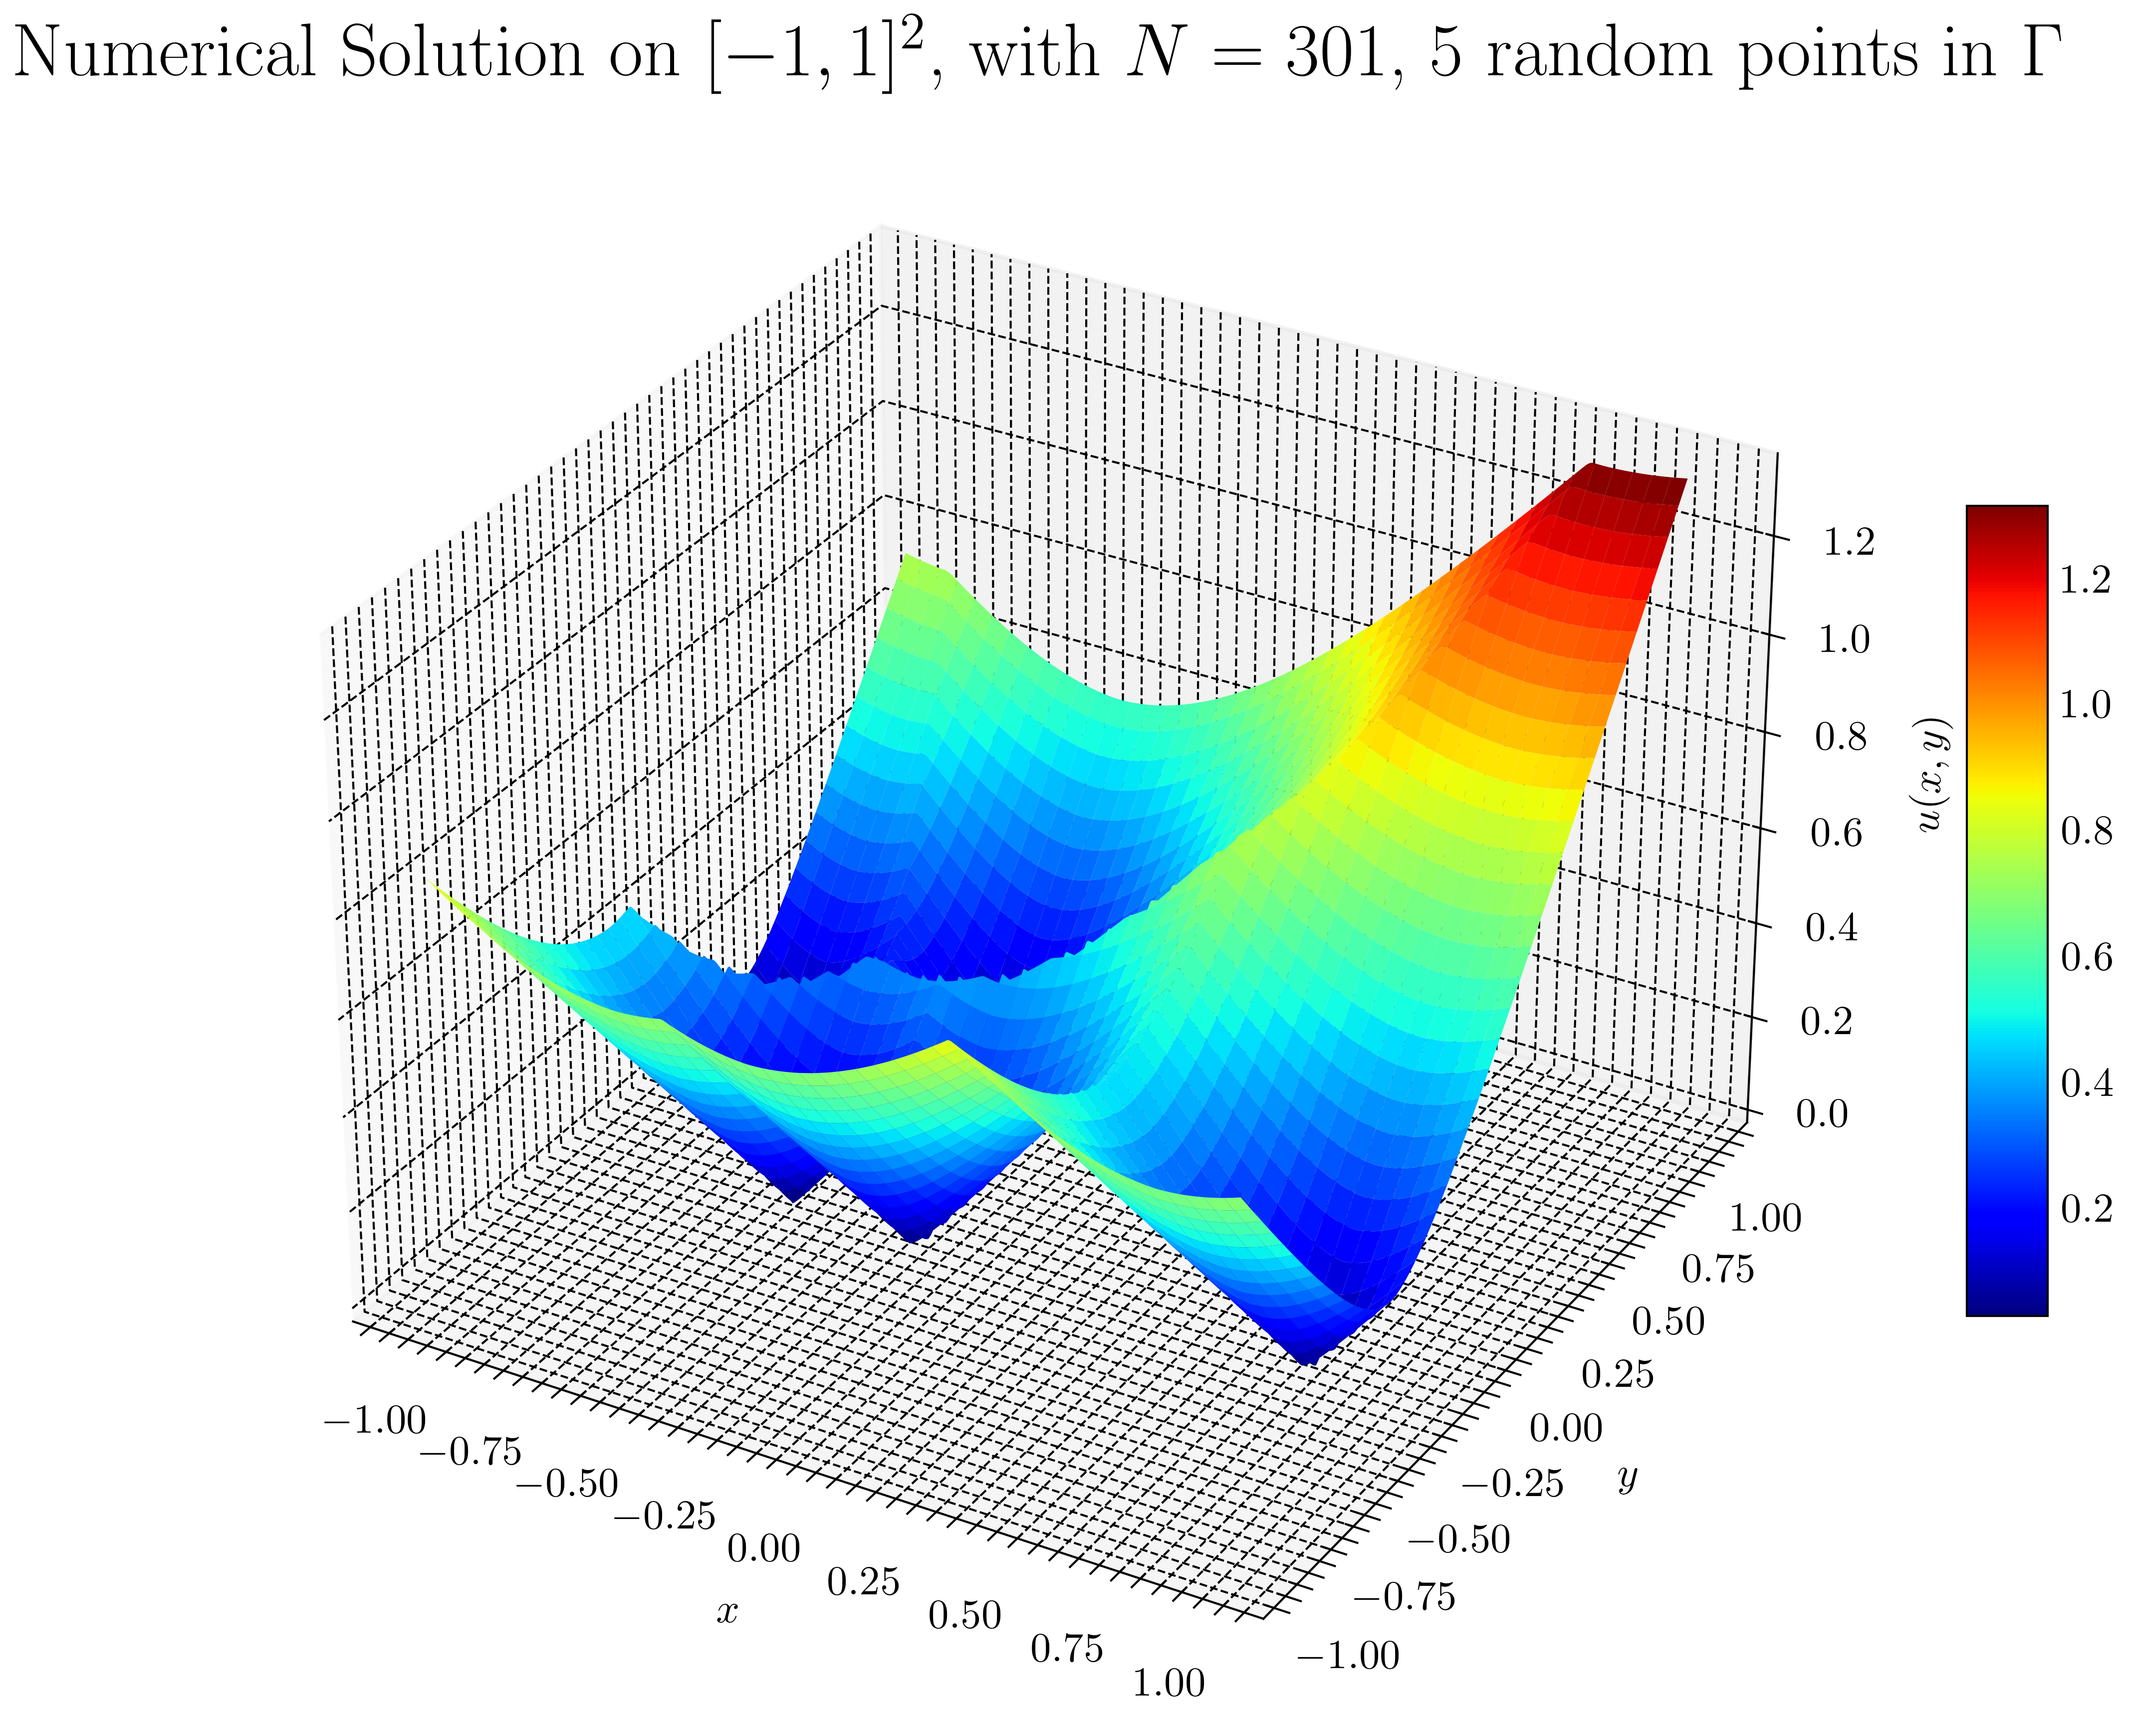
\includegraphics[width=0.7\textwidth]{plots/solution_3d_surface_random5.png} % Replace with your own logo or image
    \vfill
    \vspace{0.8cm}
    {\large \today\par}
\end{titlepage}

%----------------------------------------------------------------------------------------
%    TABLE OF CONTENTS (OPTIONAL)
%----------------------------------------------------------------------------------------

\tableofcontents
\thispagestyle{empty}

\clearpage

\section{Introduction}
%this is where you will describe the problem (e.g. previous work, related work,...) you are solving and the objectives
\label{sec:intro}
The Eikonal equations have several applications across many fields of mathematics, engineering, and others. They are particularly used for solving optimization problems, as we will see in this project. These equations associated to some side-condition, are of the form \\
\begin{equation}
\label{original-eikonal}
    \begin{cases}
        \|\nabla u(\textbf{x})\|_2=f(\textbf{x}) , \quad\textbf{x} \in\R^n\\
        u(\textbf{x})=\phi(\textbf{x}),\quad \textbf{x} \in \Gamma \subset \R^n
    \end{cases}
\end{equation}
where $\|\cdot\|_2$ denotes the Euclidean norm in $\R^n$, and $u,f,\phi:\R^n\xrightarrow{}\R$. Alternatively, we can rewrite \eqref{original-eikonal} as 
\begin{equation}
    \begin{cases}
        \sum_{i=1}^{n}\big(\frac{\partial u}{\partial x_i}\big)^2=f^2(\textbf{x}) , \quad\textbf{x} \in\R^n\\
        u(\textbf{x})=\phi(\textbf{x}),\quad \textbf{x} \in \Gamma \subset \R^n
    \end{cases}
\end{equation}

\noindent In this report, we will focus on solving the Eikonal equation in 2 space dimensions. We will use the discretization and fast-sweeping method proposed by Zhao in 2008. Before this, we will present some interpretations of the meaning of $u(x,y)$, as well as a use of our solution for optimal path planning.

\section{Theory}
%Introduce the equation and give some details
\subsection{2D Distance function}
An important application of Eikonal functions is the computation of Euclidean distances in $\R^n$. In particular, let us consider the following problem : suppose that we are given a  finite set of points $\Gamma = \{\gamma^{(1)},\dots,\gamma^{(m)}\}$, and for each $\textbf{x}=(x,y)$ in our computational domain, we would like to compute the shortest distance to $\Gamma$. Hence, we would like to have a function $d(x,y)$ such that
\begin{equation}
\label{min-problem}
    d(\textbf{x}) = \min_{\gamma \in \Gamma}\|\textbf{x}-\gamma\|_2
\end{equation}
Consider this problem in $\R^2$, if we let $(x,y)$ such that its closest point in $\Gamma$ is some point $\gamma^{*}=(\gamma_1,\gamma_2)$, which is the unique minimizer of \eqref{min-problem}, then:
\begin{gather*}
    d(x,y) = \sqrt{(x-\gamma_1)^2+(y-\gamma_2)^2} \\[10pt] 
    \implies\frac{\partial d}{\partial x}=\frac{x-\gamma_1}{\sqrt{(x-\gamma_1)^2+(y-\gamma_2)^2}}, \quad 
    \frac{\partial d}{\partial y}=\frac{y-\gamma_2}{\sqrt{(x-\gamma_1)^2+(y-\gamma_2)^2}} \\[10pt] 
    \implies \|\nabla d(x,y)\|^{2}_{2} = \Bigg(\frac{\partial d}{\partial x}\Bigg)^2 + \Bigg(\frac{\partial d}{\partial y}\Bigg)^2=1
\end{gather*}
Indeed, $d(x,y)$ solves the Eikonal equation where $f(x,y) \equiv 1$, and naturally we have $d(x,y)=\phi(x,y)=0$ where $(x,y)\in\Gamma$ (the distance to the boundary is 0 when the point lies on the boundary).
\section{Numerical methods}
\subsection{Discretization and scheme}
%this is where you present your numerical method/scheme. You may additionally put accuracy, stability in here. Also talk about the implementation details here.
H. Zhao proposed the fast-sweeping method in ?? to solve Eikonal equations numerically. His proposed the following discretization, which uses Gauss-Seidel iterations. In 2 dimensions, given a space step $h$, the proposed scheme is:

\begin{equation*}
    ((u_{i,j}-u_{xmin})^{+})^2+((u_{i,j}-u_{ymin})^{+})^2 = f_{i,j}^{2}h^2
\end{equation*}

\noindent where
\begin{itemize}
    \item $(x)^{+} = \max(x,0)$
    \item $u_{i,j}\approx u(ih,jh)$, $u_{xmin} = \min\{u_{i-1,j},u_{i+1,j}\}$ and $u_{ymin} = \min\{u_{i,j-1},u_{i,j+1}\}$
\end{itemize}

\noindent Figure \ref{fig:graph_discretization} shows a visualization of the scheme. The updates of the points $u_{i,j}$ must be done by "sweeping" the domain in all 4 possible directions (or $2^d$ directions in $\mathbb{R}^d$), after having initialized a grid. Without loss of generality, the sweeps in 2 dimensions can be done as follows, assuming a square domain:
\begin{itemize}
    \item \textbf{Sweep 1 : } Start from the bottom-left corner of the domain, updating the points from left to right. Hence, the last point updated is the top-right corner one.
    \item \textbf{Sweep 2 : } Start from the bottom-right corner of the domain, updating the points from right to left. This gets us to the last point updated being the top-left corner one.
    \item  \textbf{Sweep 3 : } Start from the top-left corner of the domain, updating from left to right. Similarly, the last point to be updated is the bottom-right corner one
    \item \textbf{Sweep 4 : } Last possible direction. Start from top-right corner of the domain, updating the points from right to left. The last point to be updated is the bottom left corner.
\end{itemize}

\begin{figure}[h!]
    \centering
    \begin{tikzpicture}
        % Draw the grid points
        \foreach \x in {0,1,2} {
            \foreach \y in {0,1,2} {
                \filldraw (\x,\y) circle (3pt);
            }
        }

        % Highlight the center point (i,j)
        \filldraw[red] (1,1) circle (2pt) node[above right] {$(i,j)$};

        % Draw the stencil neighbors
        \filldraw[blue] (0,1) circle (2pt) node[left] {$(i-1,j)$};
        \filldraw[blue] (2,1) circle (2pt) node[right] {$(i+1,j)$};
        \filldraw[blue] (1,0) circle (2pt) node[below] {$(i,j-1)$};
        \filldraw[blue] (1,2) circle (2pt) node[above] {$(i,j+1)$};

        % Draw lines connecting the stencil points
        \draw[thick] (1,1) -- (0,1);
        \draw[thick] (1,1) -- (2,1);
        \draw[thick] (1,1) -- (1,0);
        \draw[thick] (1,1) -- (1,2);
    \end{tikzpicture}
    \caption{Discretization for the Fast-Sweeping method in 2D}
    \label{fig:graph_discretization}
\end{figure}

Hence, the iteration can be written as follows:
\begin{itemize}
    \item \textbf{(1)} Initialize the computational domain by setting all points to a large value $M$ (this value should be larger than the largest value of the solution $u$ in the domain).
    \item \textbf{(2)} Place the boundary conditions $\Gamma=\{\gamma_1,\dots,\gamma_m\}$ on the domain. These points are fixed and should never be updated!
    \item \textbf{(3)} Apply a batch of sweeps to the domain, i.e. sweeps 1 to 4. If needed, sweep again the domain until convergence is met. To monitor convergence, compute at the $k$-th sweep $E = \max\limits_{i,j} \left| u_{i,j}^{(k)} - u_{i,j}^{(k-1)} \right|$ where $u_ {i,j}^{(k)}$ denotes the solution on the stencil $(i,j)$ after the $k$-th sweep.
\end{itemize}

\subsection{Code implementation}
We implement the fast-sweeping method in Python using the \texttt{numpy} library \ref{}. All the scripts are available in the GitHub repository available in the introduction \ref{}. \\
We replicate domains with the help of a class named \texttt{computational\_domain}
, equipped with the method \texttt{ComputationalDomain(N,a,b,c,d)} which instantiates an object with several attributes, including the attribute \texttt{grid} which is an $N\times N$ \texttt{Numpy} 2D array, representing the square $[a,b]\times[c,d]\subset\R^2$. The constructor of the class sets the initial value $M$ described above in section \ref{} to 100, but can be chosen by the user.\\
This class is also equipped with the method \texttt{Gamma(coordinates)} which sets the boundary conditions in the domain. \texttt{coordinates} must be a list of 2D coordinates given as a indices, for example \texttt{coordinates = [(0,0), (1,0), (4,4)]}. Note that this method assumed Python indexing. For example, the code below would help create the following domain: \\
\begin{lstlisting}[language=Python, caption=Instance of computational domain, label=lst:fsweep]
from computational_domain import ComputationalDomain
domain = ComputationalDomain(N = 6, a = -1, b = 1, c = -1, d = 1)
domain.Gamma([(0,0), (2,1), (4,3), (1,4)])
print(domain.grid)
\end{lstlisting} \\

$$\[
\begin{bmatrix}
0 & 100 & 100 & 100 & 100 & 100 \\
100 & 100 & 100 & 100 & 0 & 100 \\
100 & 0 & 100 & 100 & 100 & 100 \\
100 & 100 & 100 & 100 & 100 & 100 \\
100 & 100 & 100 & 0 & 100 & 100 \\
100 & 100 & 100 & 100 & 100 & 100
\end{bmatrix}
\]$$


\section{Results}
\subsection{2D Distance function}
As argued above in part \ref{}, the Eikonal equation can be used to compute the shortest distance to a boundary $\Gamma \subset \R^n$. Therefore, we test our implementation for the BVP:
\begin{equation}
\label{cone_bvp}
    \begin{cases}
        \|\nabla u(\textbf{x})\|_2=1 , \quad\textbf{x} \in[-1,1]^2\\
        u(0,0)=0
    \end{cases}
\end{equation}
The solution to this BVP is the 2D cone, given by $u(x,y)=\sqrt{x^2+y^2}$. Therefore, we can easily compare our numerical solution to the analytic one, and study its convergence as well.
For the analysis below, we discretize the square $[-1,1]^2$ evenly with $N=257 \implies h \approx 0.0078$. The solution is obtained after monitoring the convergence of the sweeps : we sweep the domain until the $L_{\infty}$ norm of change between the current grid and the previous one is less than $\epsilon=10^{-6}$
\begin{figure}[h!]
    \centering
    \begin{minipage}{0.48\linewidth}
        \centering
        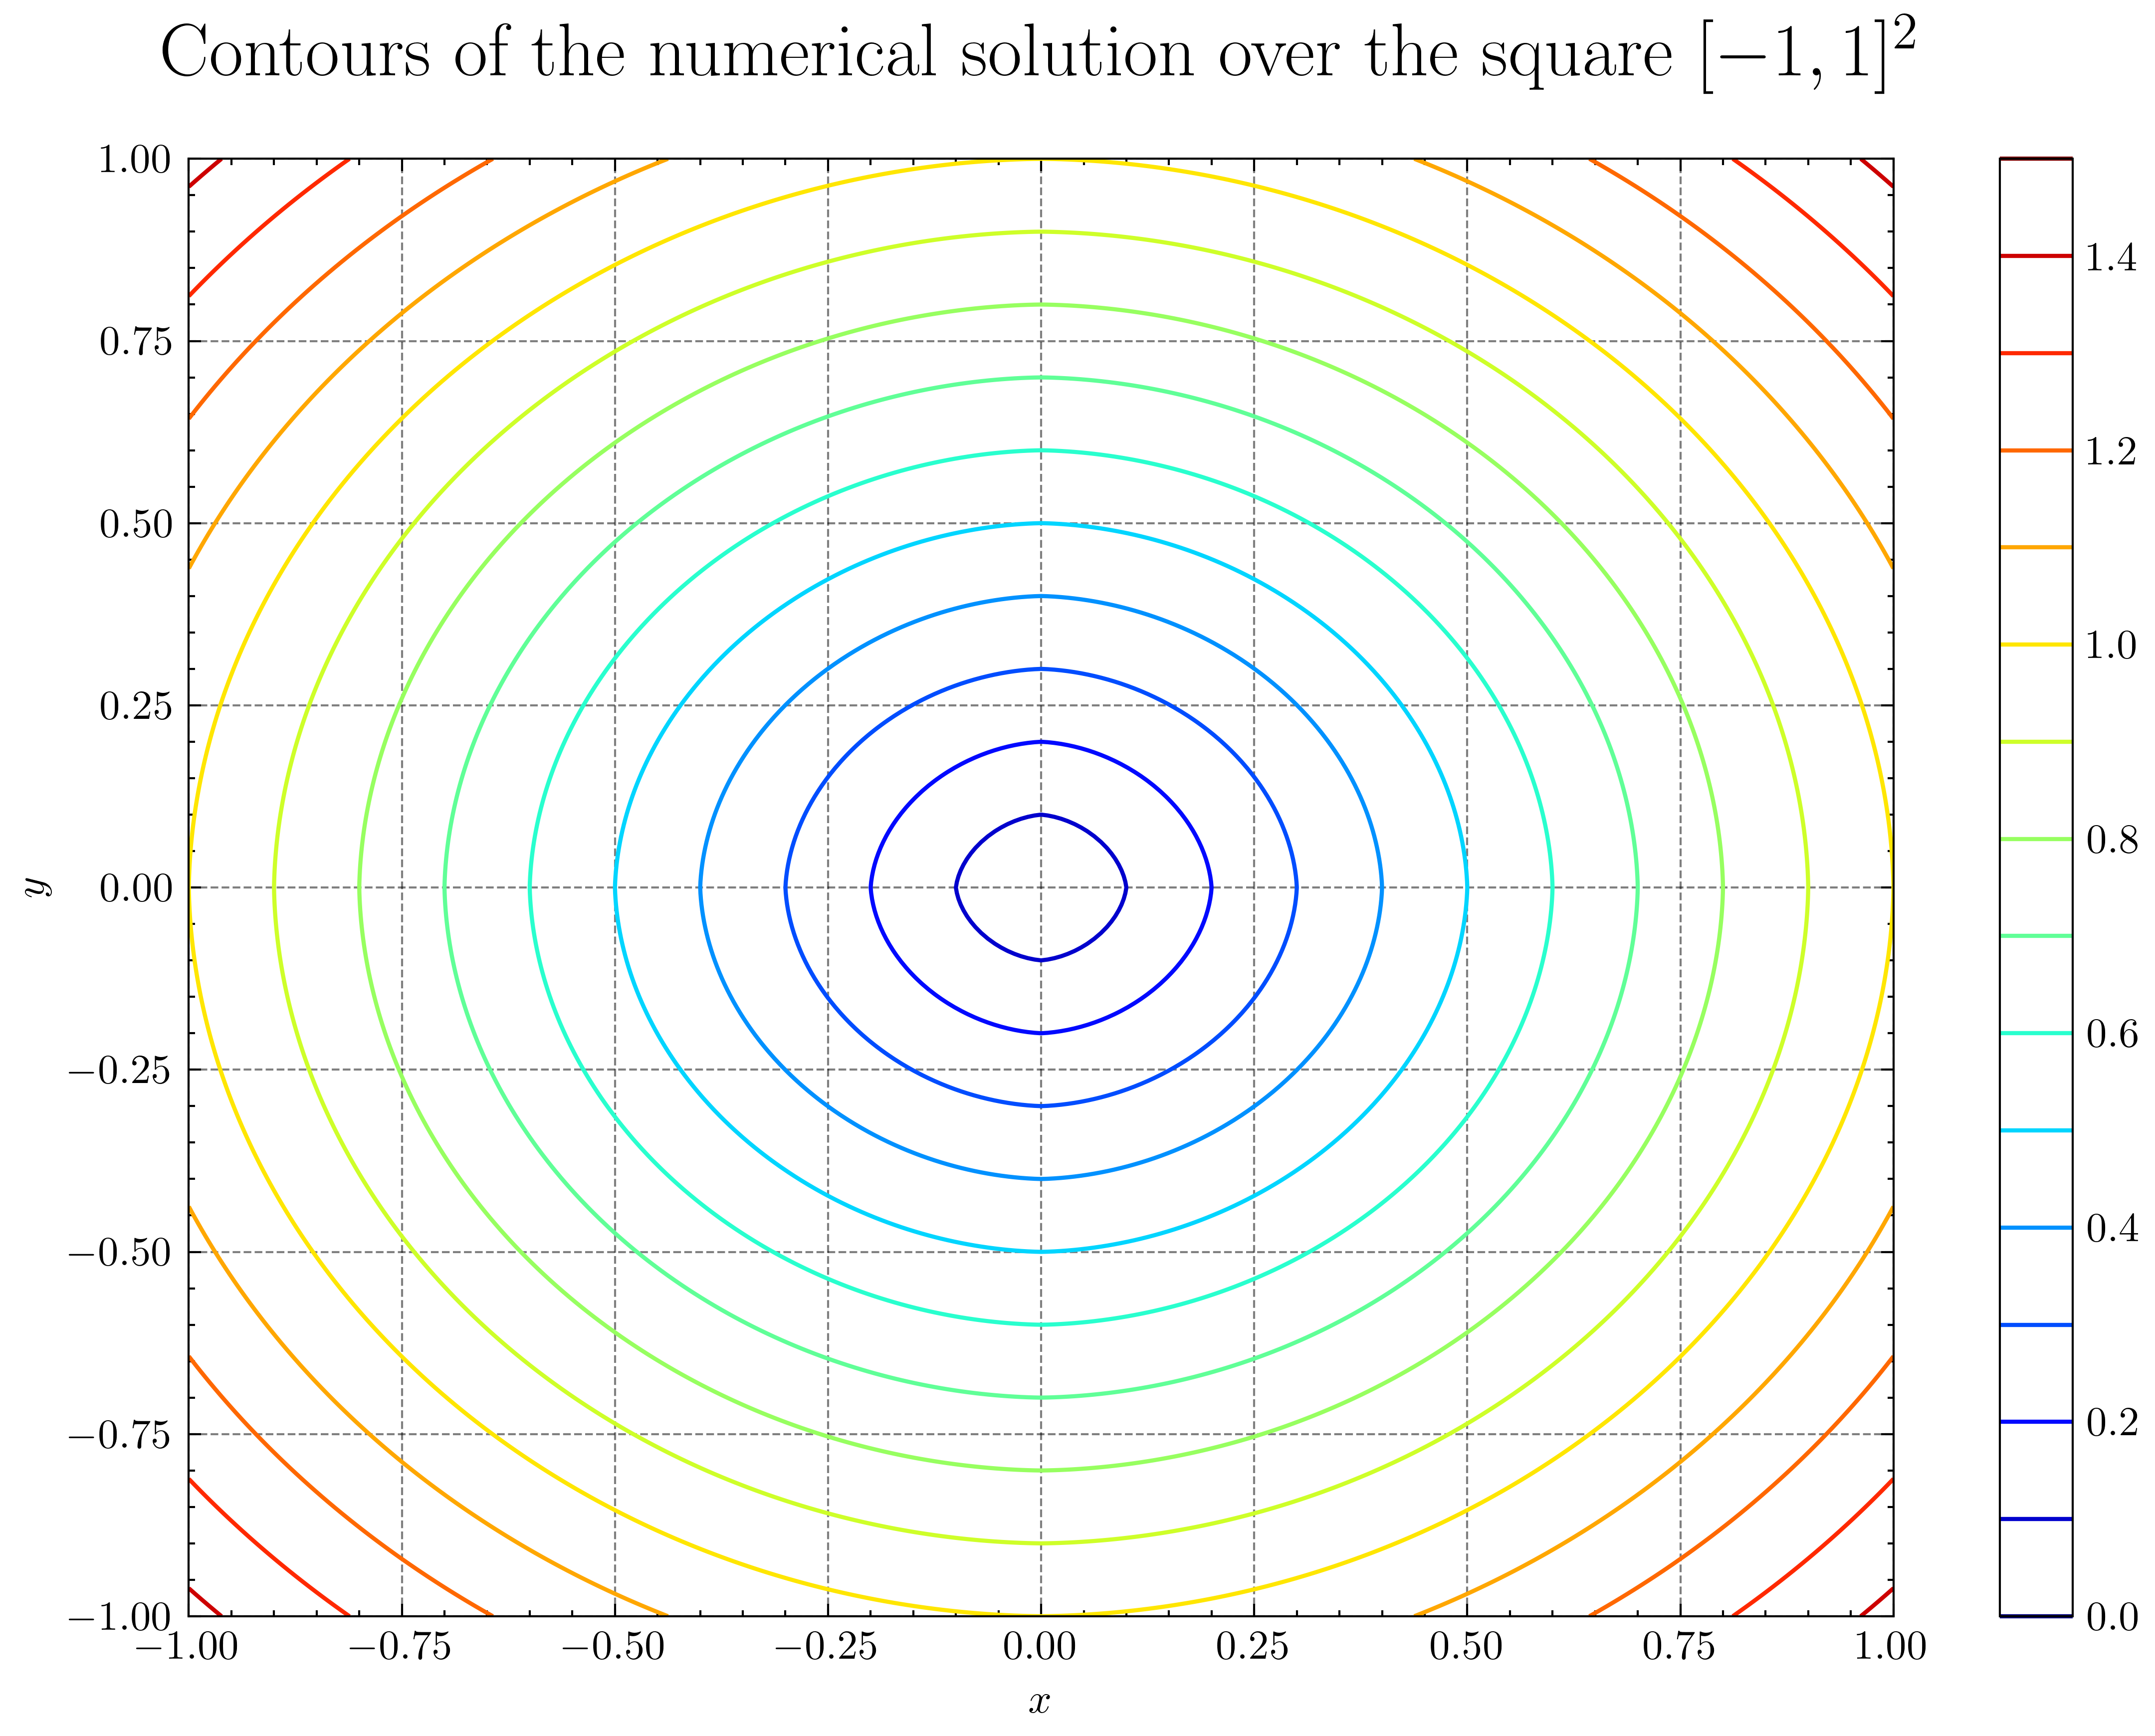
\includegraphics[width=\linewidth]{plots/contour_plot_2D_distance.png}
        \caption{Contour plot of 2D distance.}
        \label{fig:contour-distance}
    \end{minipage}
    \hfill
    \begin{minipage}{0.48\linewidth}
        \centering
        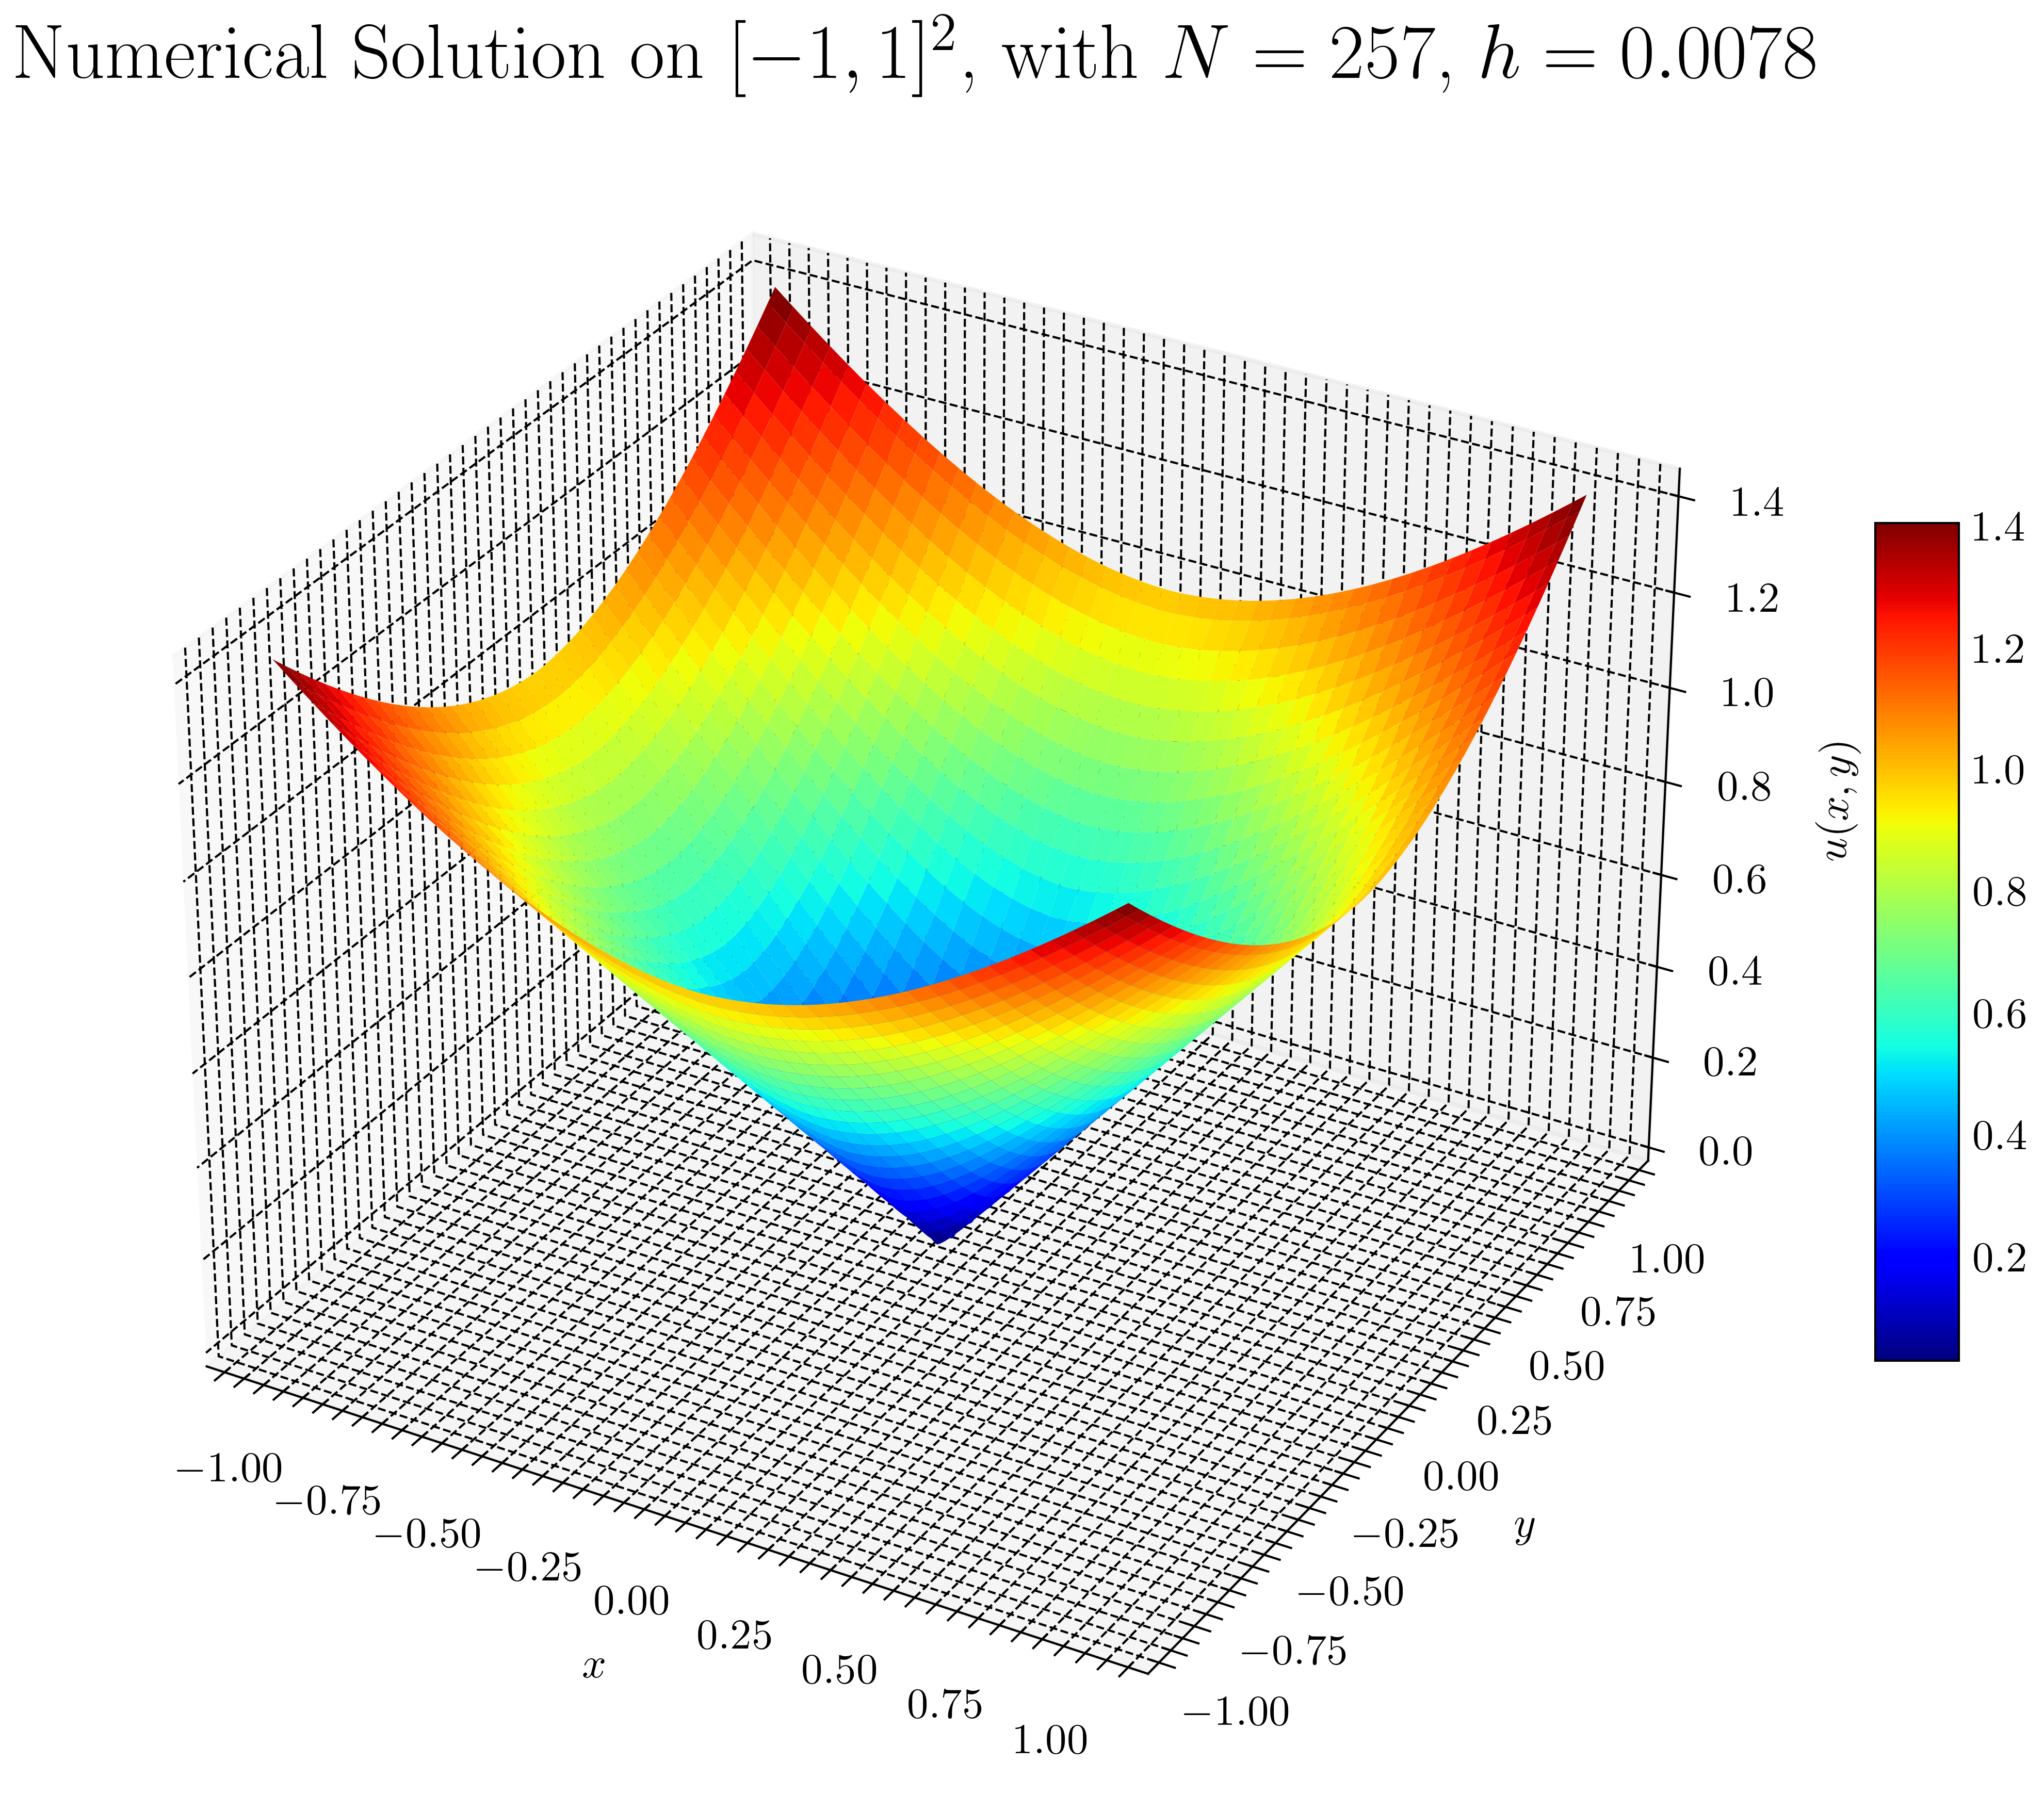
\includegraphics[width=\linewidth]{plots/solution_3d_surface.png}
        \caption{3D surface of the distance function.}
        \label{fig:3d-surface}
    \end{minipage}
\end{figure}
\vspace{20pt}

\noindent Finally, we can analyze the convergence of the scheme for the solution above. As described by Zhao in \ref{}, the accuracy of the fast sweeping method is of order $O(|h\log h|)$. On the plot below, we can see that the fast-sweeping method we implemented indeed converges to the true function $u(x,y)=\sqrt{x^2+y^2}$ at the rate $O(|h\log h|)$


\begin{figure}[h]
  \centering
  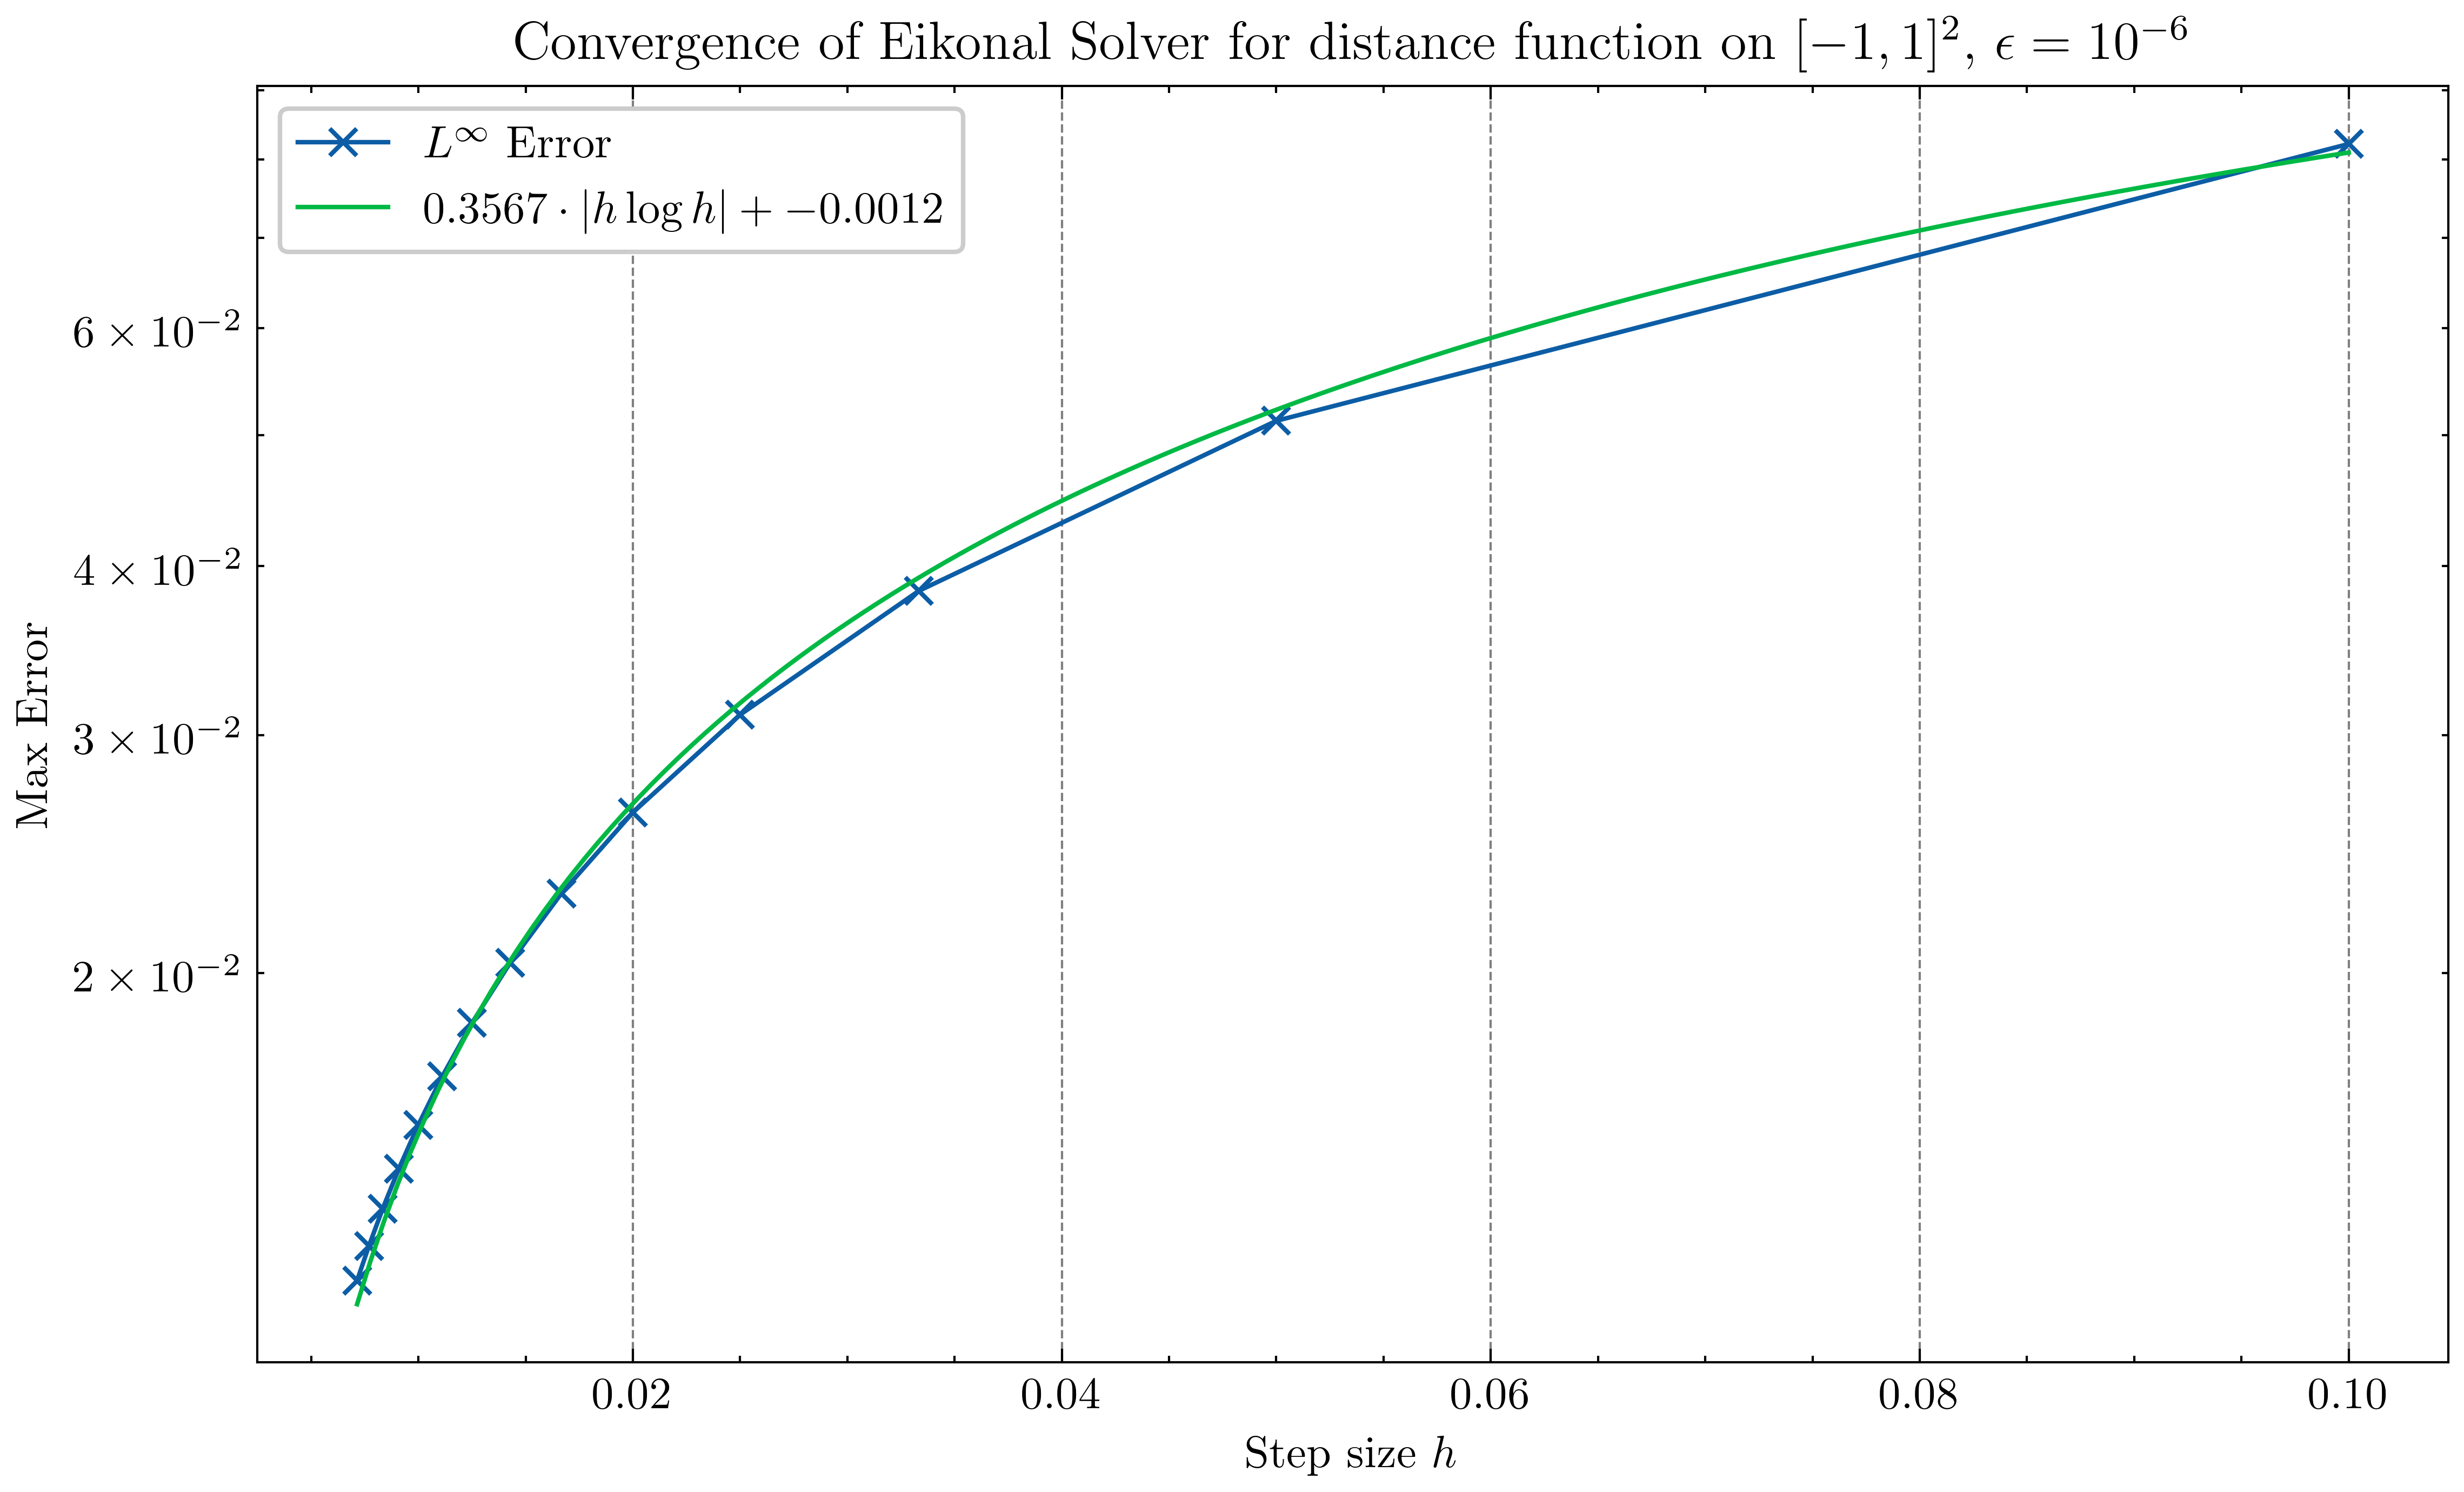
\includegraphics[width=0.7\linewidth]{plots/convergence2d_step_size.png}
  \caption{Accuracy of the fast-sweeping method for the distance function to the origin}
  \label{fig:error_distance}
\end{figure}

\subsubsection{Distance function with several boundary points}
The example in the previous subsection was only considering one boundary value at the origin of the domain, i.e. the set $\Gamma$ was simply $\Gamma=\{(0,0)\}$. We can introduce several other boundary points, and the solution $u$ picked up by the fast sweeping-method will give at any point $(x,y)$ the distance to the closest point $\gamma\in\Gamma$, as we showed in section \ref{}. Indeed consider the case below, where we chose 5 points at random on $[-1,1]^2$, and set these points to be 0 in the domain. Our Eikonal solver then converges to the numerical solution $u(x,y)$ whose contours and 3D surface are given by figures x and x respectively.

\vspace{5pt}

\begin{figure}[h]
  \centering
  \begin{minipage}{0.45\textwidth}
    \centering
    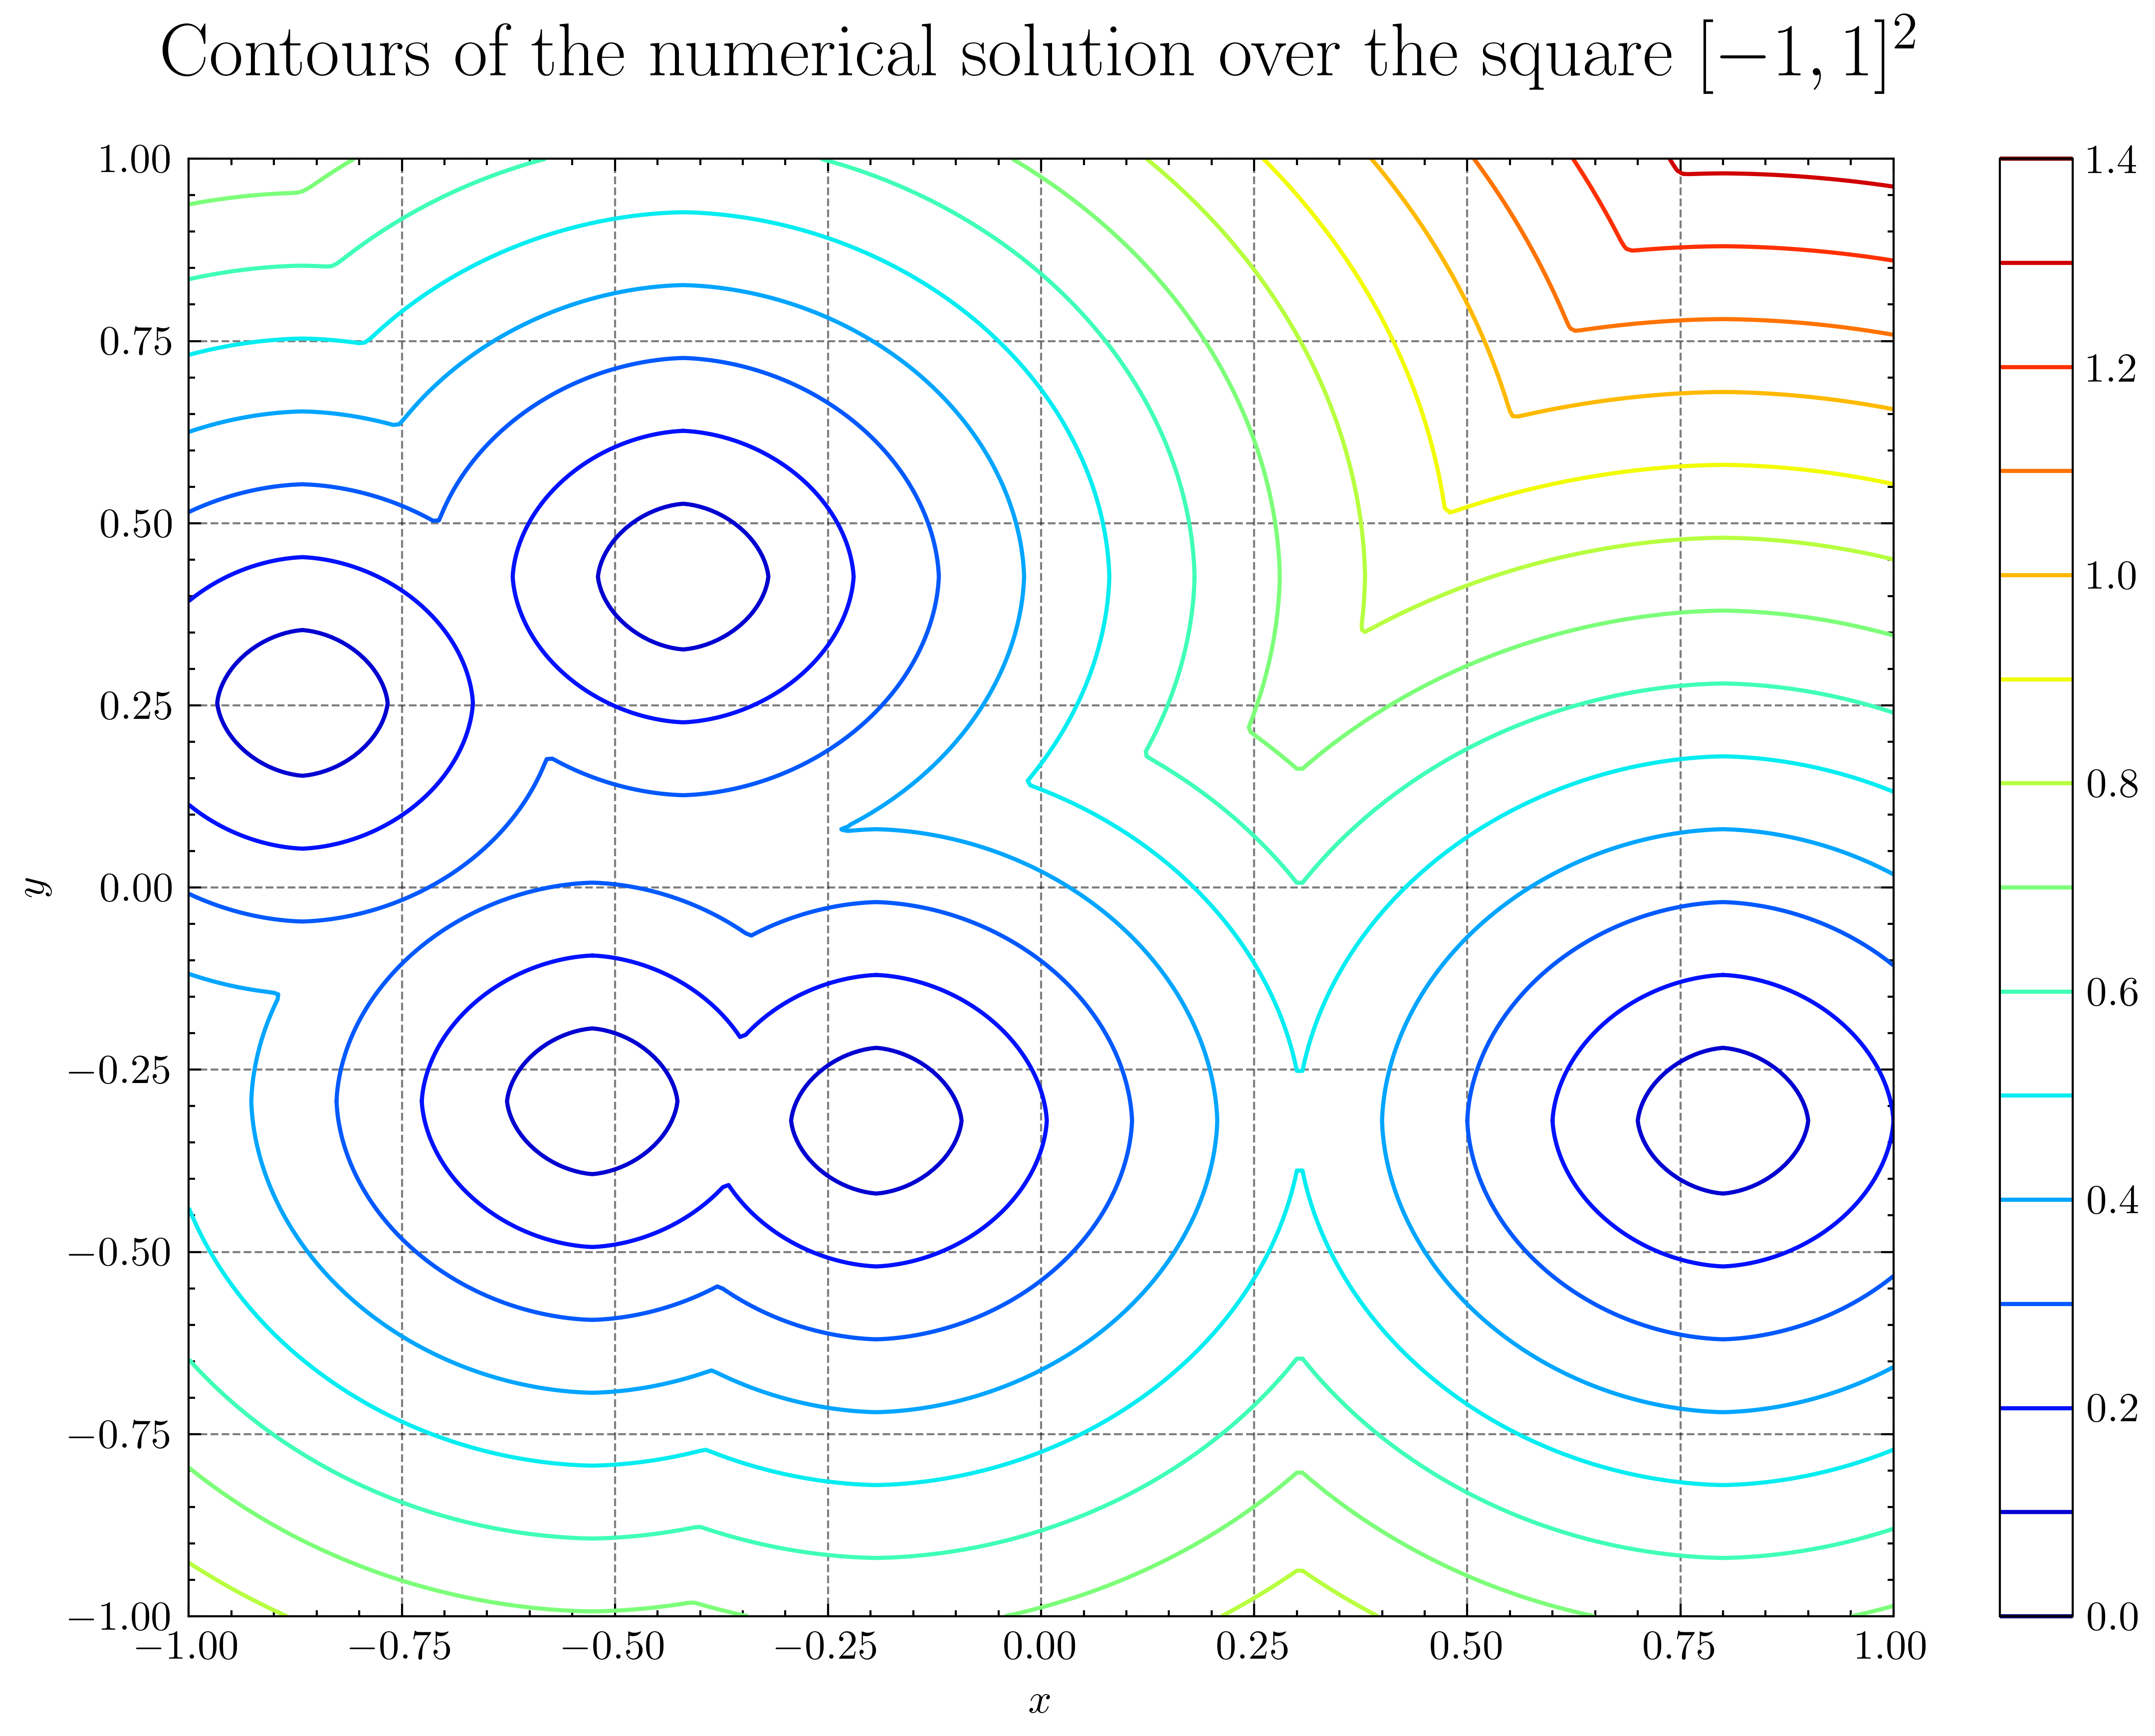
\includegraphics[width=\linewidth]{plots/contour_plot_random5.png}
    \caption{Contours of numerical solution ($|\Gamma|=5$)}
    \label{fig:contour5}
  \end{minipage}
  \hfill
  \begin{minipage}{0.45\textwidth}
    \centering
    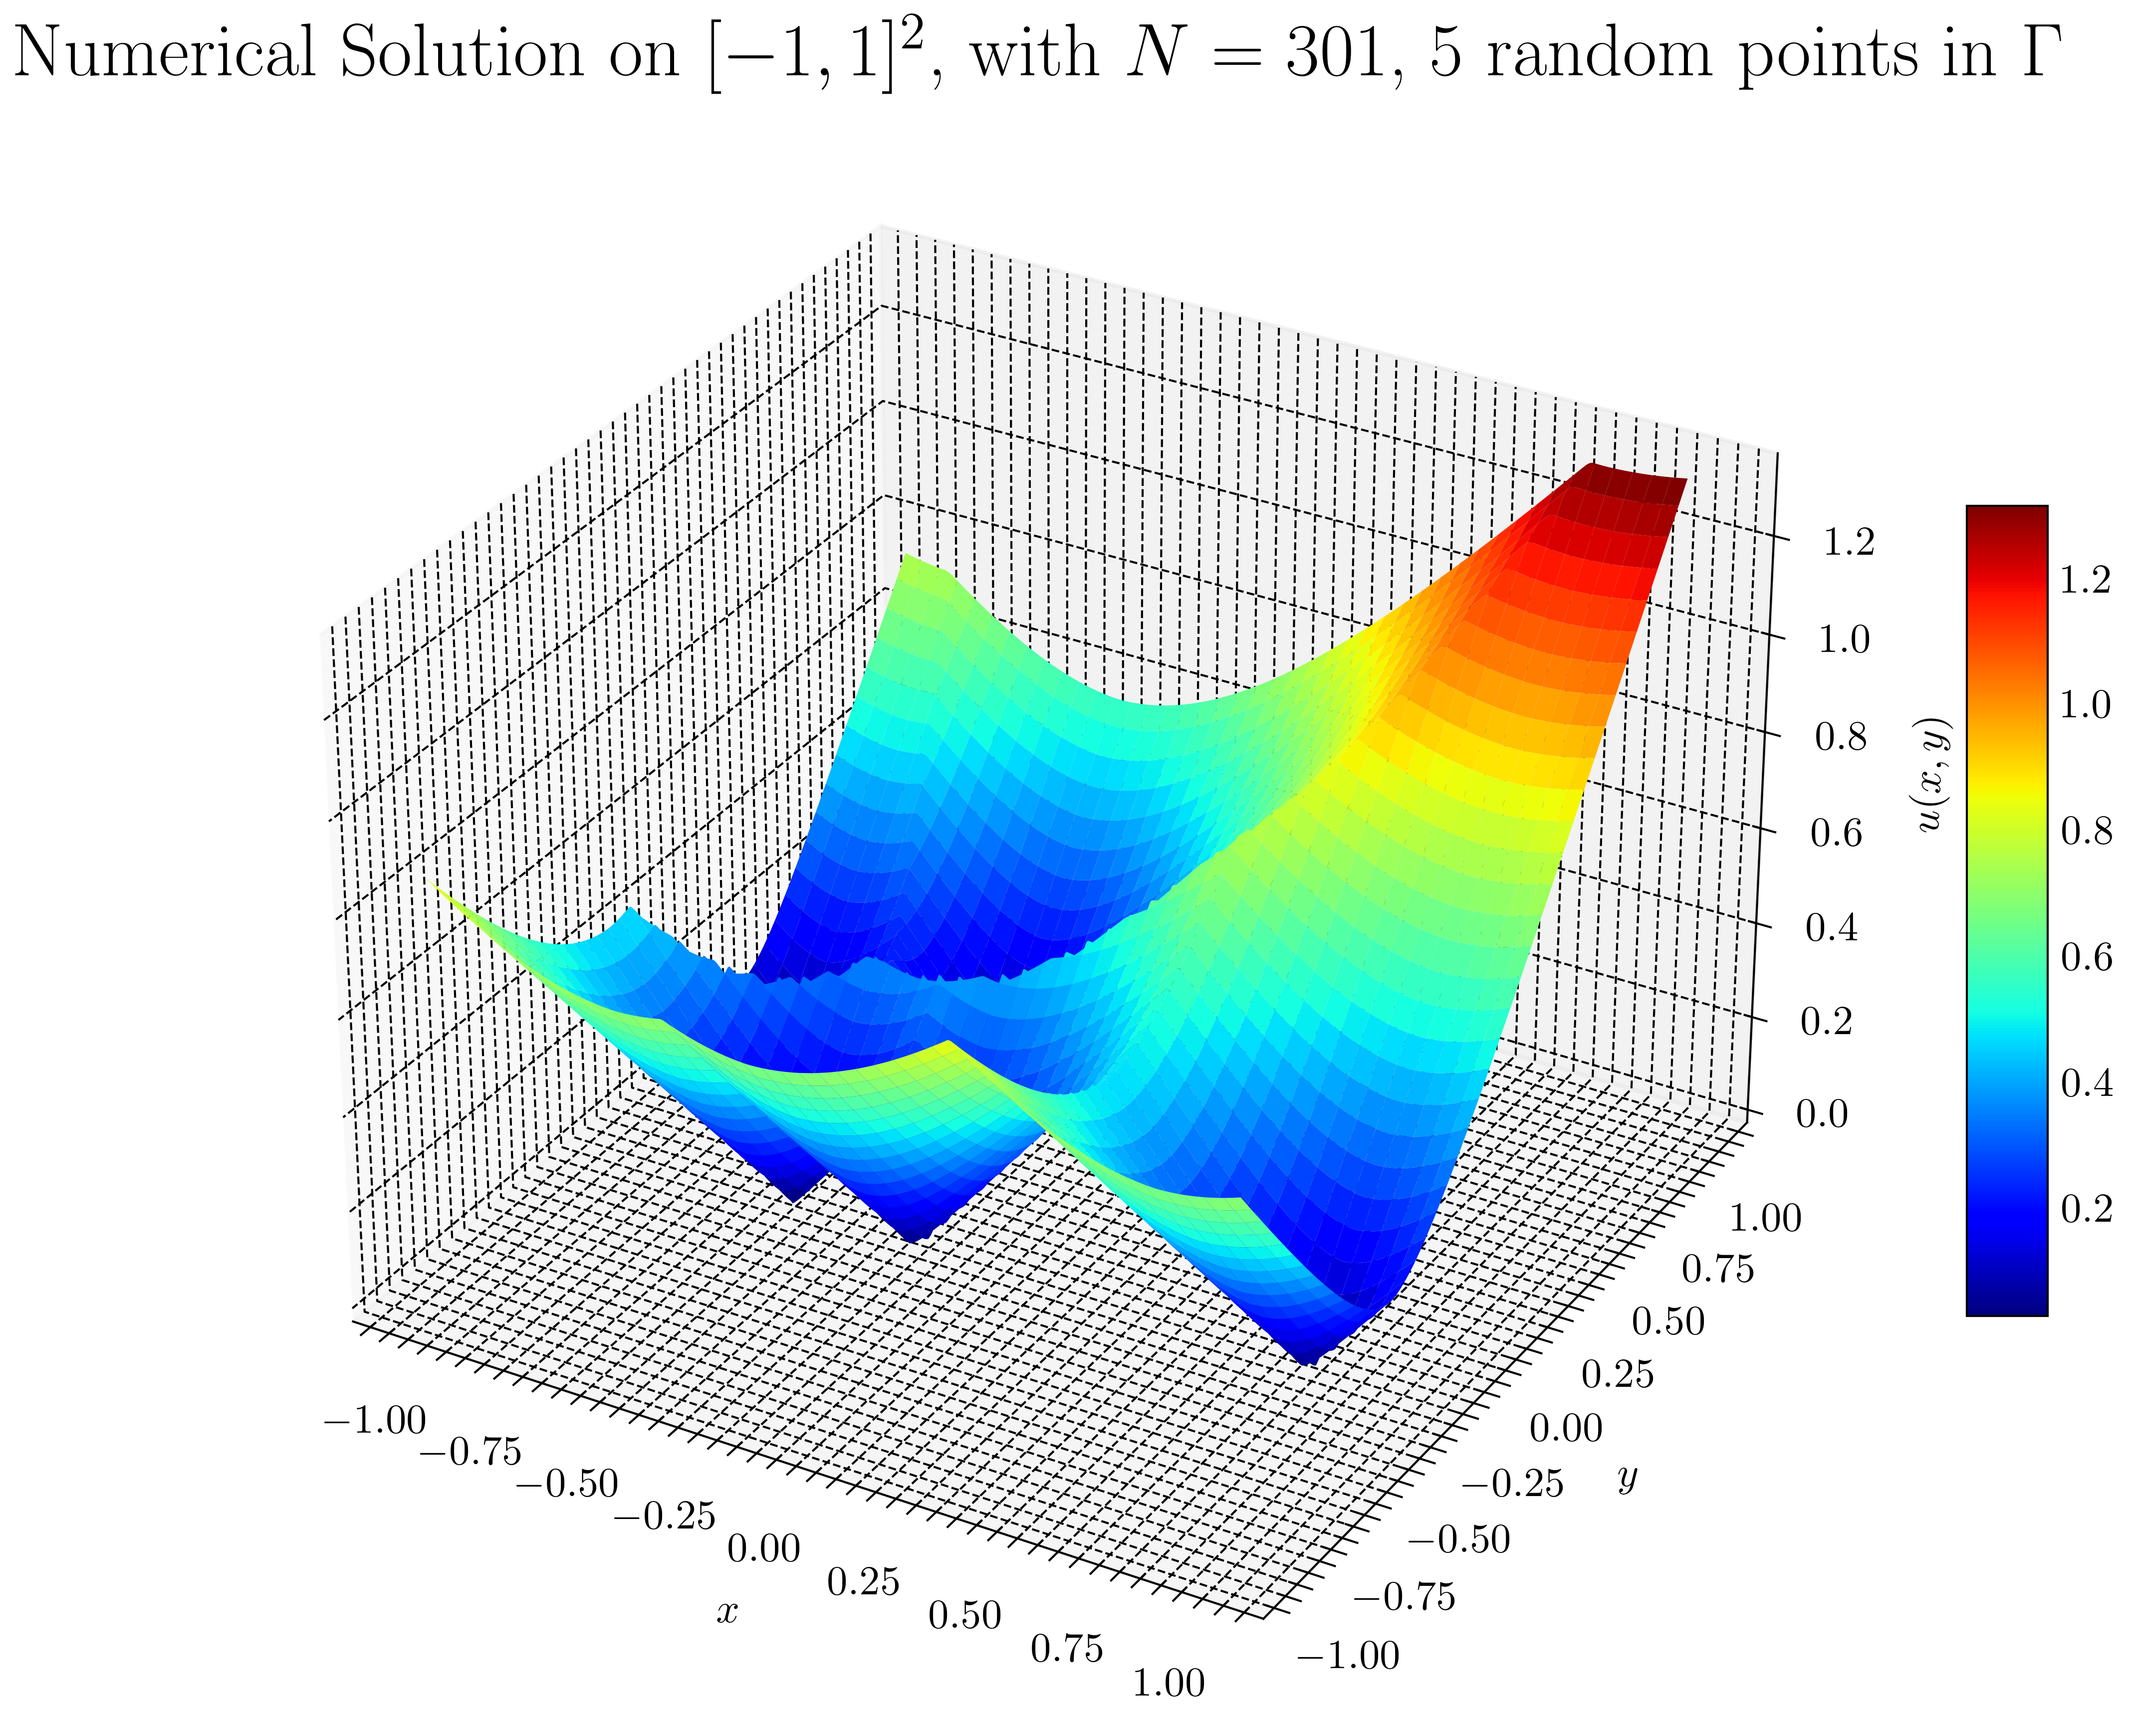
\includegraphics[width=\linewidth]{plots/solution_3d_surface_random5.png}
    \caption{3D surface of the solution ($|\Gamma$|=5)}
    \label{fig:surface5}
  \end{minipage}
\end{figure}

\vspace{5pt}
\noindent Finally, we look at another case where we introduce several more boundary points in $\Gamma$. In the example below, we sampled uniformly at random 30 points in $[-1,1]^2$ and set these points to have value 0. A heatmap of the solution is:

\begin{figure}[h!]
  \centering
  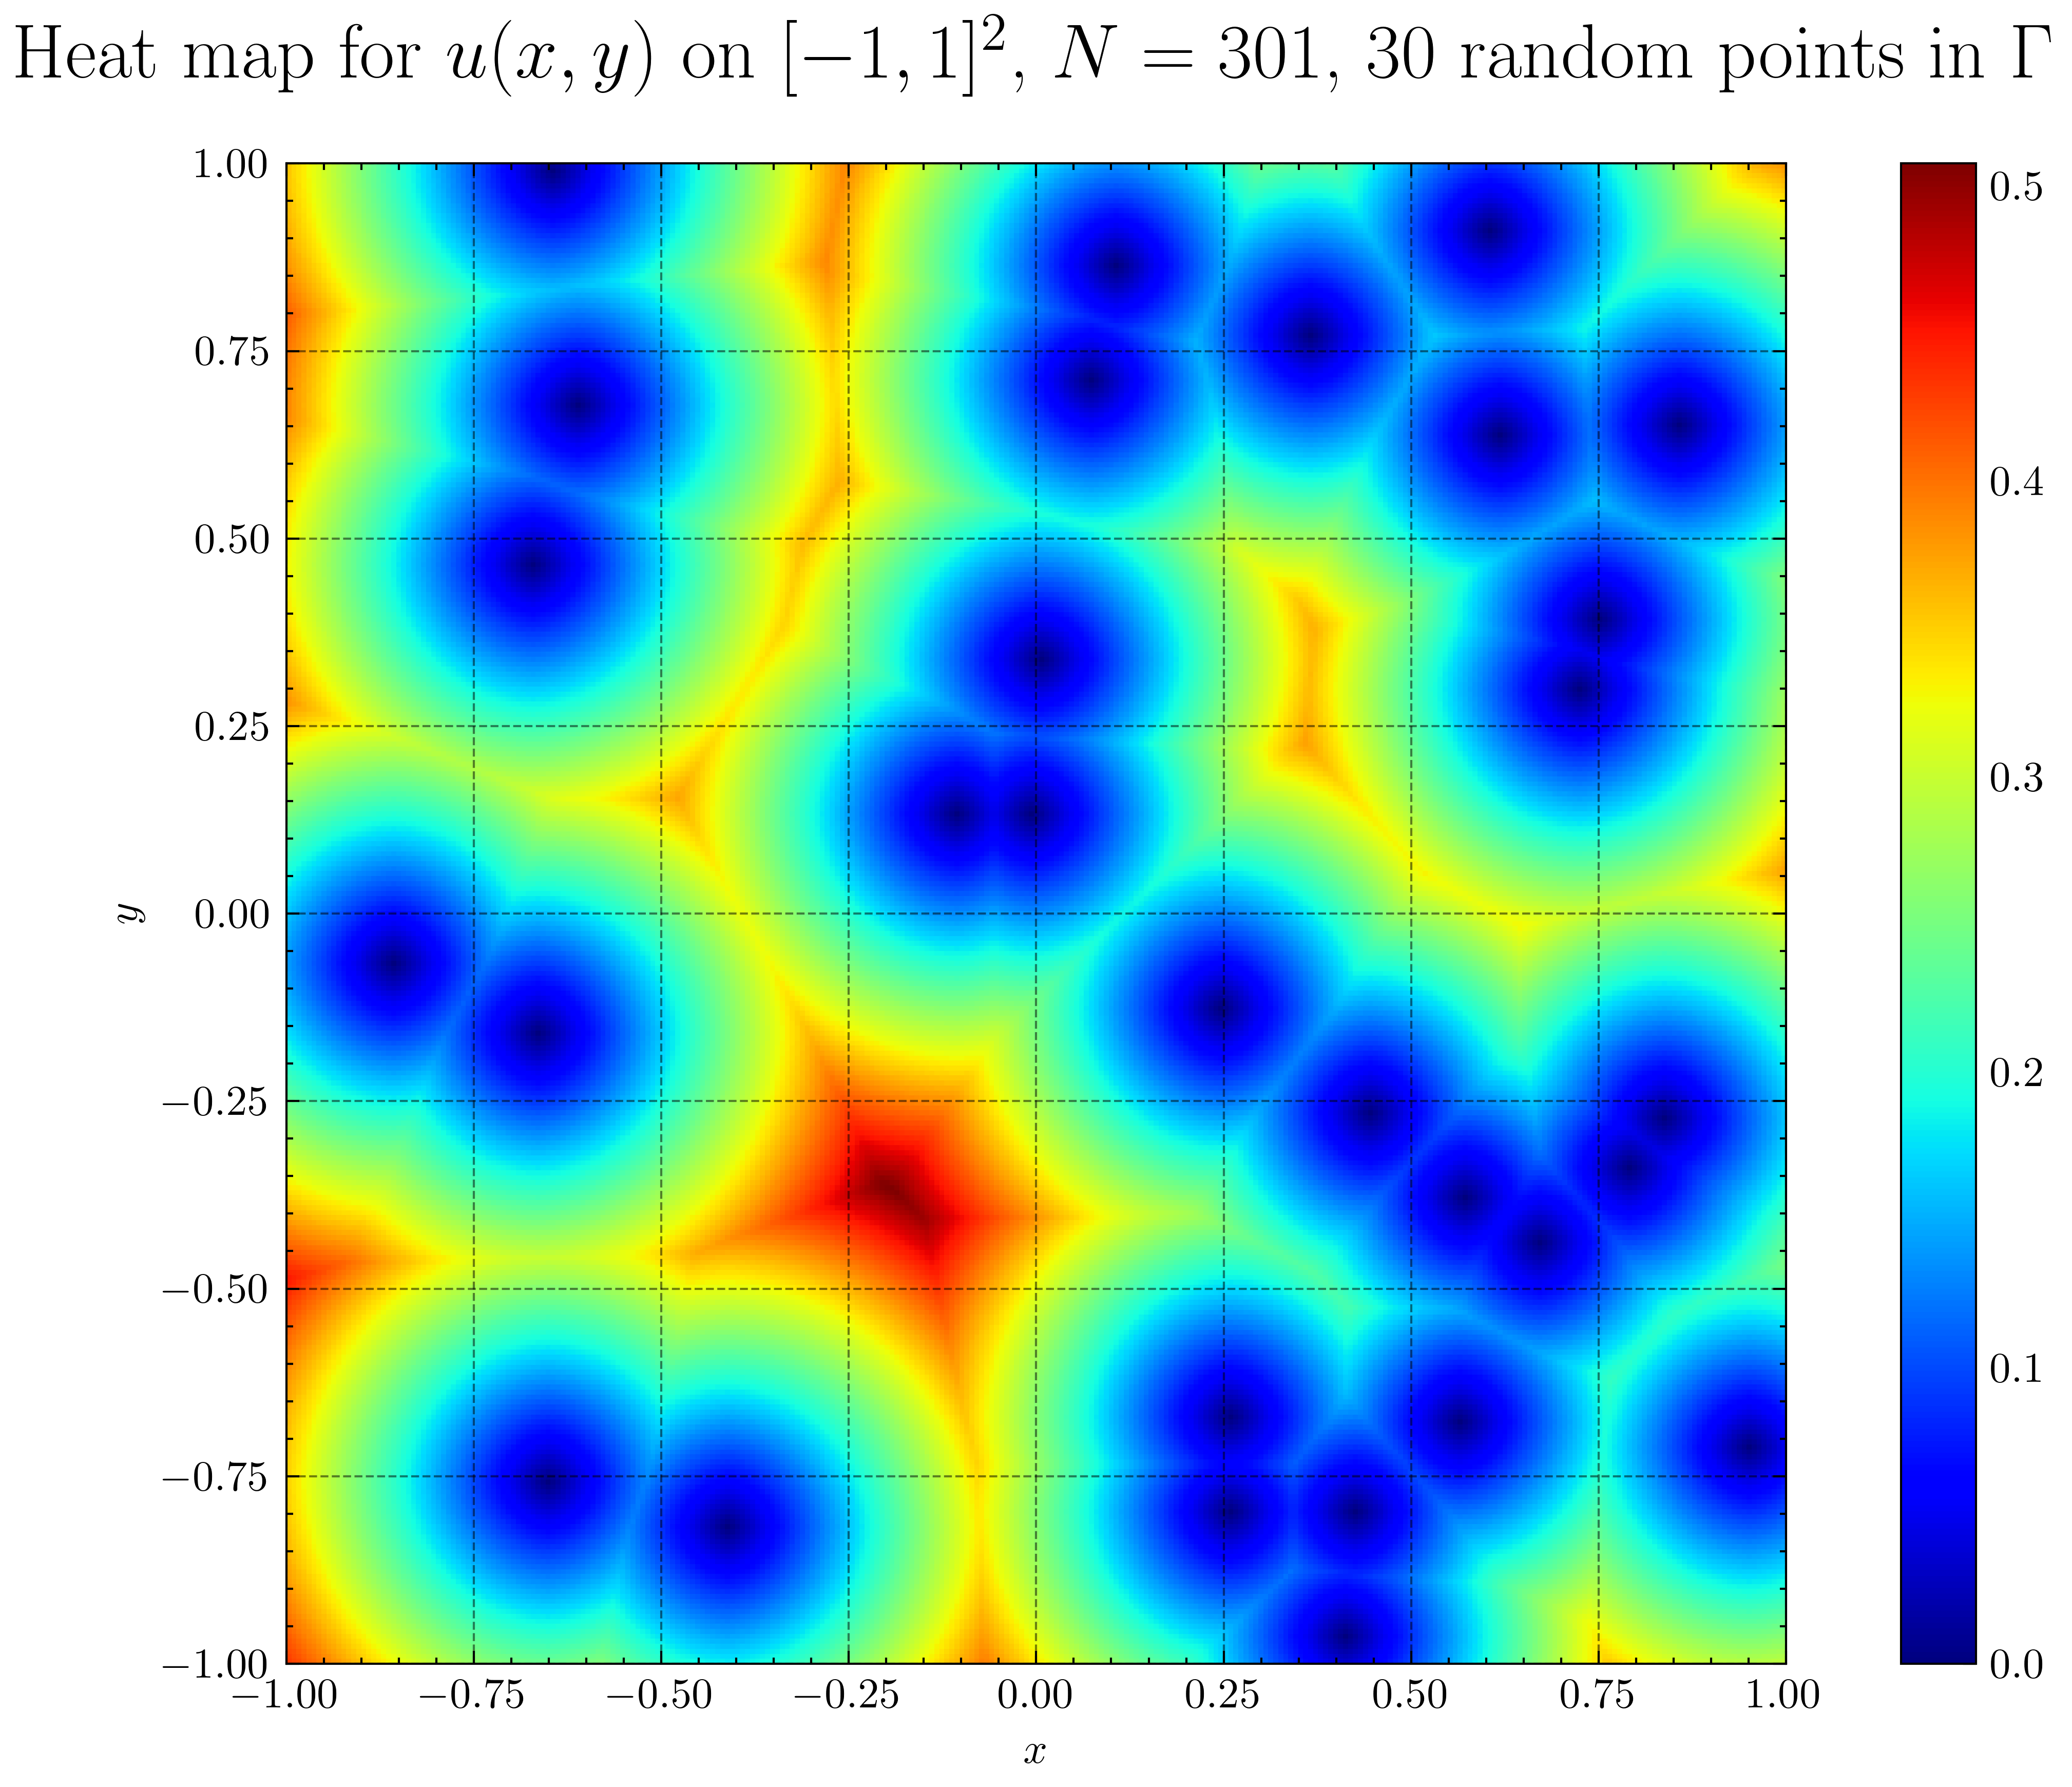
\includegraphics[width=0.5\textwidth]{plots/heatmap_random30.png}
  \caption{Your image caption}
  \label{fig:heatmap30random}
\end{figure}

\newpage

\subsection{General Eikonal equations}
In this subsection, we now are interested at problems of the form of \ref{original-eikonal} where $f(x,y)\not\equiv 1$ on the domain. Conveniently, we will also rewrite $f(x,y)=\frac{1}{F(x,y)}$, where $F(x,y)$ can now be thought of as a velocity over the domain. As a result, the solution $u(x,y)$ does not give the distance to the boundary anymore, but rather the "cost" of the travel from $(x,y)$ to $\Gamma$.
We test our solver for the problem.

\begin{equation}
\label{arctan_equation}
    \begin{cases}
        \|\nabla u(x,y)\|_2=\frac{1}{1+0.5(x^2+y^2)} , \quad(x,y) \in [-1,1]^2 \\
        u(0,0)= 0
    \end{cases}
\end{equation}
One can easily check that $u(x,y)=\sqrt{2}\arctan\Big[\sqrt{\frac{x^2+y^2}{2}}\Big]$ solves (\ref{arctan_equation}). We use this reference to test our solver with the following parameters : $N=401$ on the discretized domain $[-1,1]^2$ which gives the step size $h=0.01$, with convergence criterion $\epsilon=10^{-6}$
\subsubsection{Convergence}
From Zhao, we know that for the general case $1/F(x,y)\not\equiv1$, the fast-sweeping method also converges to the true solution in $O(|h\log h|)$. For the reference problem defined in the section above, with $N\in\{21,41,\dots,401\}$, we get the following convergence to the true solution.

\begin{figure}[h]
  \centering
  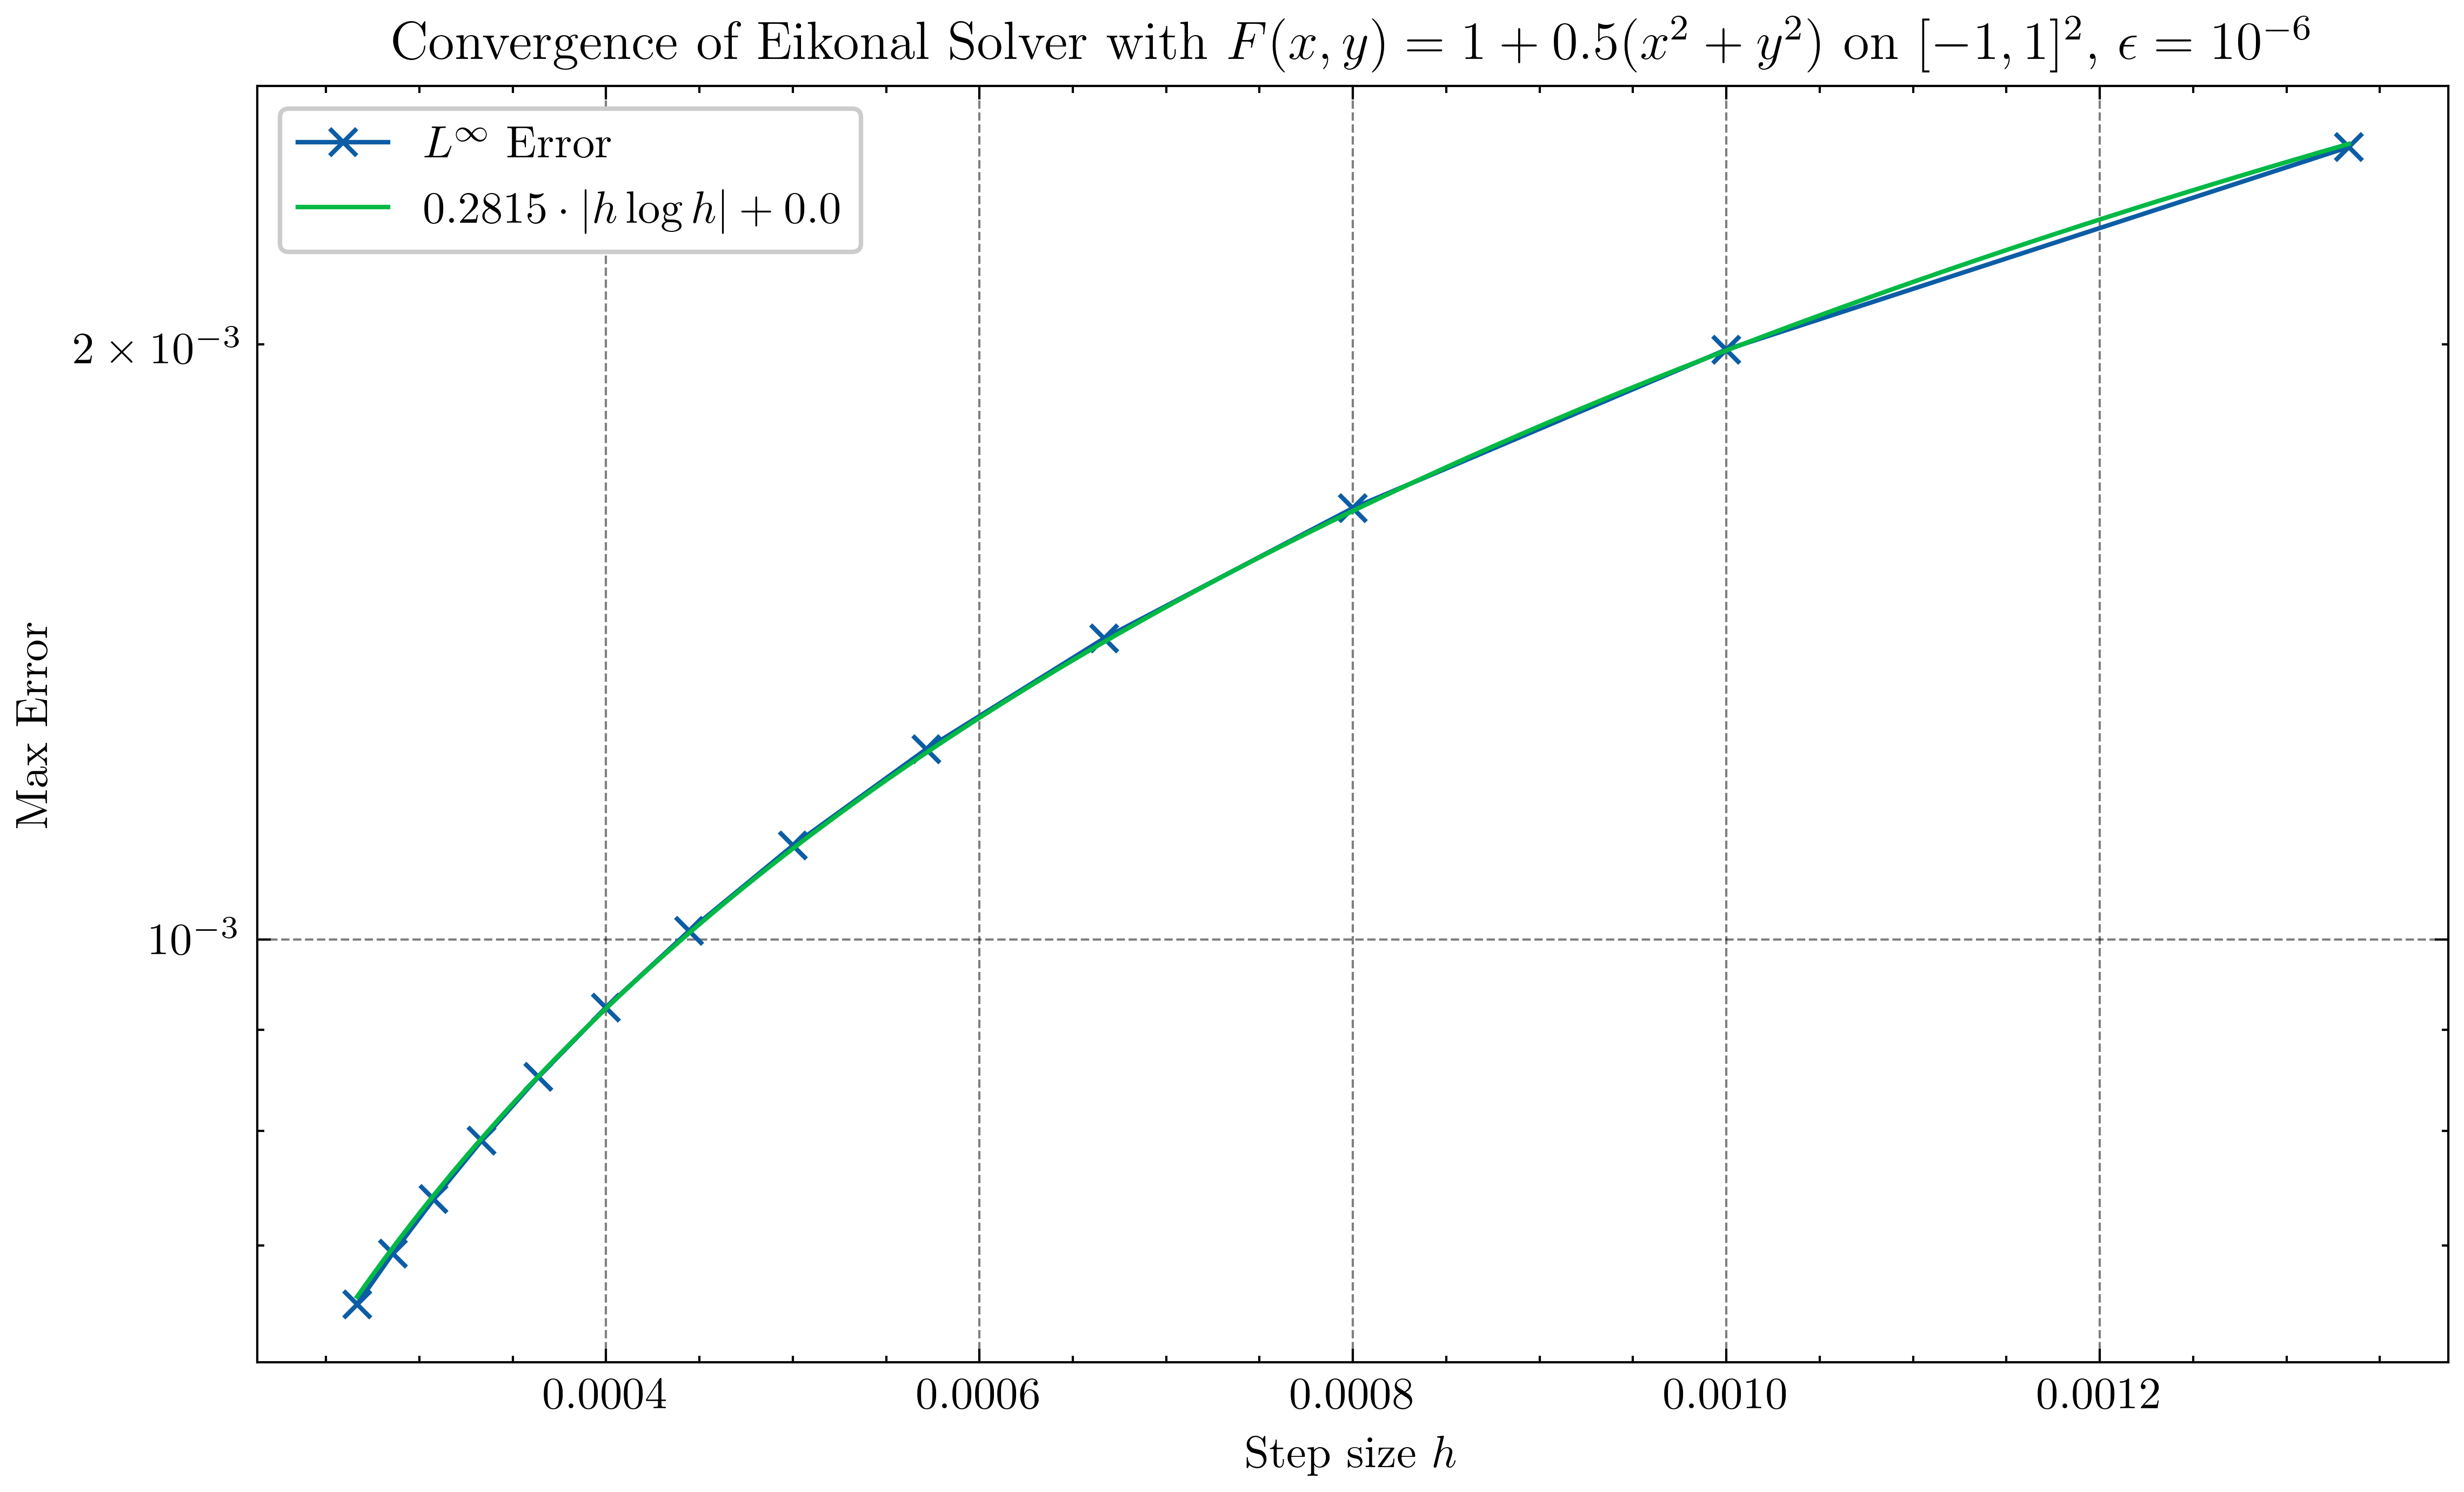
\includegraphics[width=0.6\textwidth]{plots/convergence2d_atan_step_size.png}
  \caption{Convergence plot}
  \label{fig:convarctan}
\end{figure}

\vspace{10pt}

\noindent With $N=401$, the solution looks like the following:
\begin{figure}[h]
  \centering
  \begin{minipage}{0.45\textwidth}
    \centering
    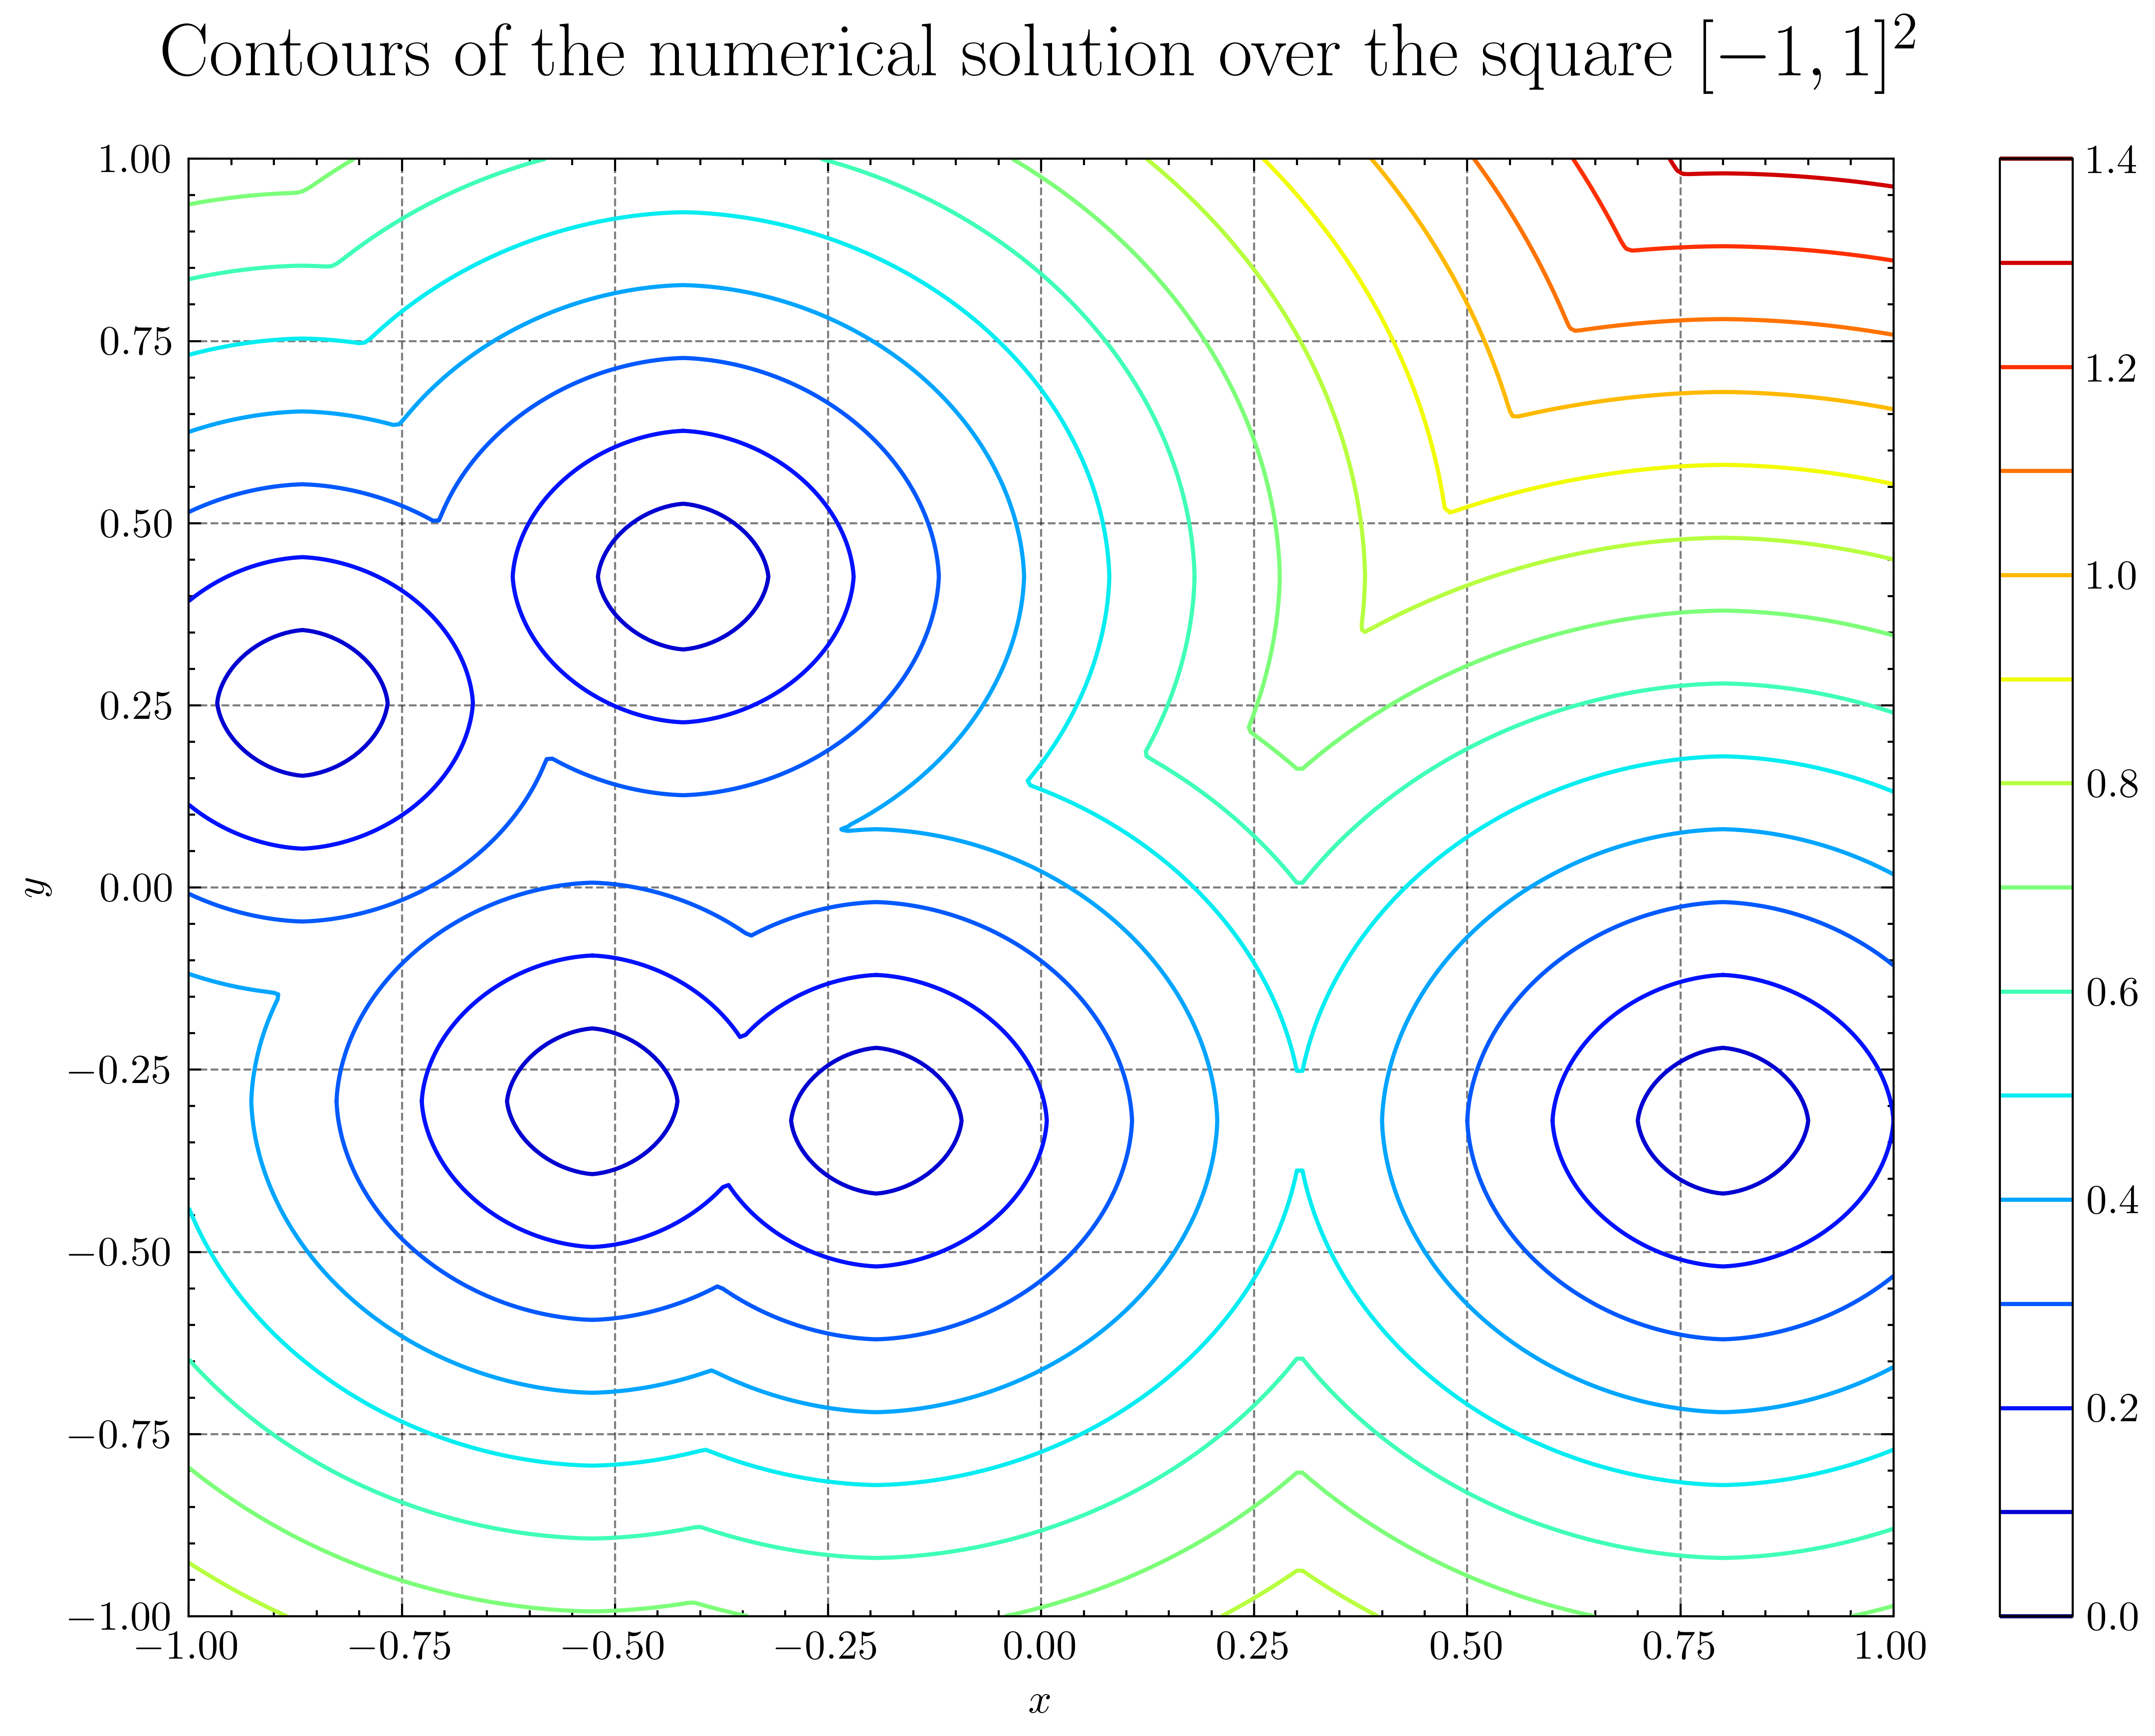
\includegraphics[width=\linewidth]{plots/contour_plot_random5.png}
    \caption{Contours of numerical solution ($|\Gamma|=5$)}
    \label{fig:contour5}
  \end{minipage}
  \hfill
  \begin{minipage}{0.45\textwidth}
    \centering
    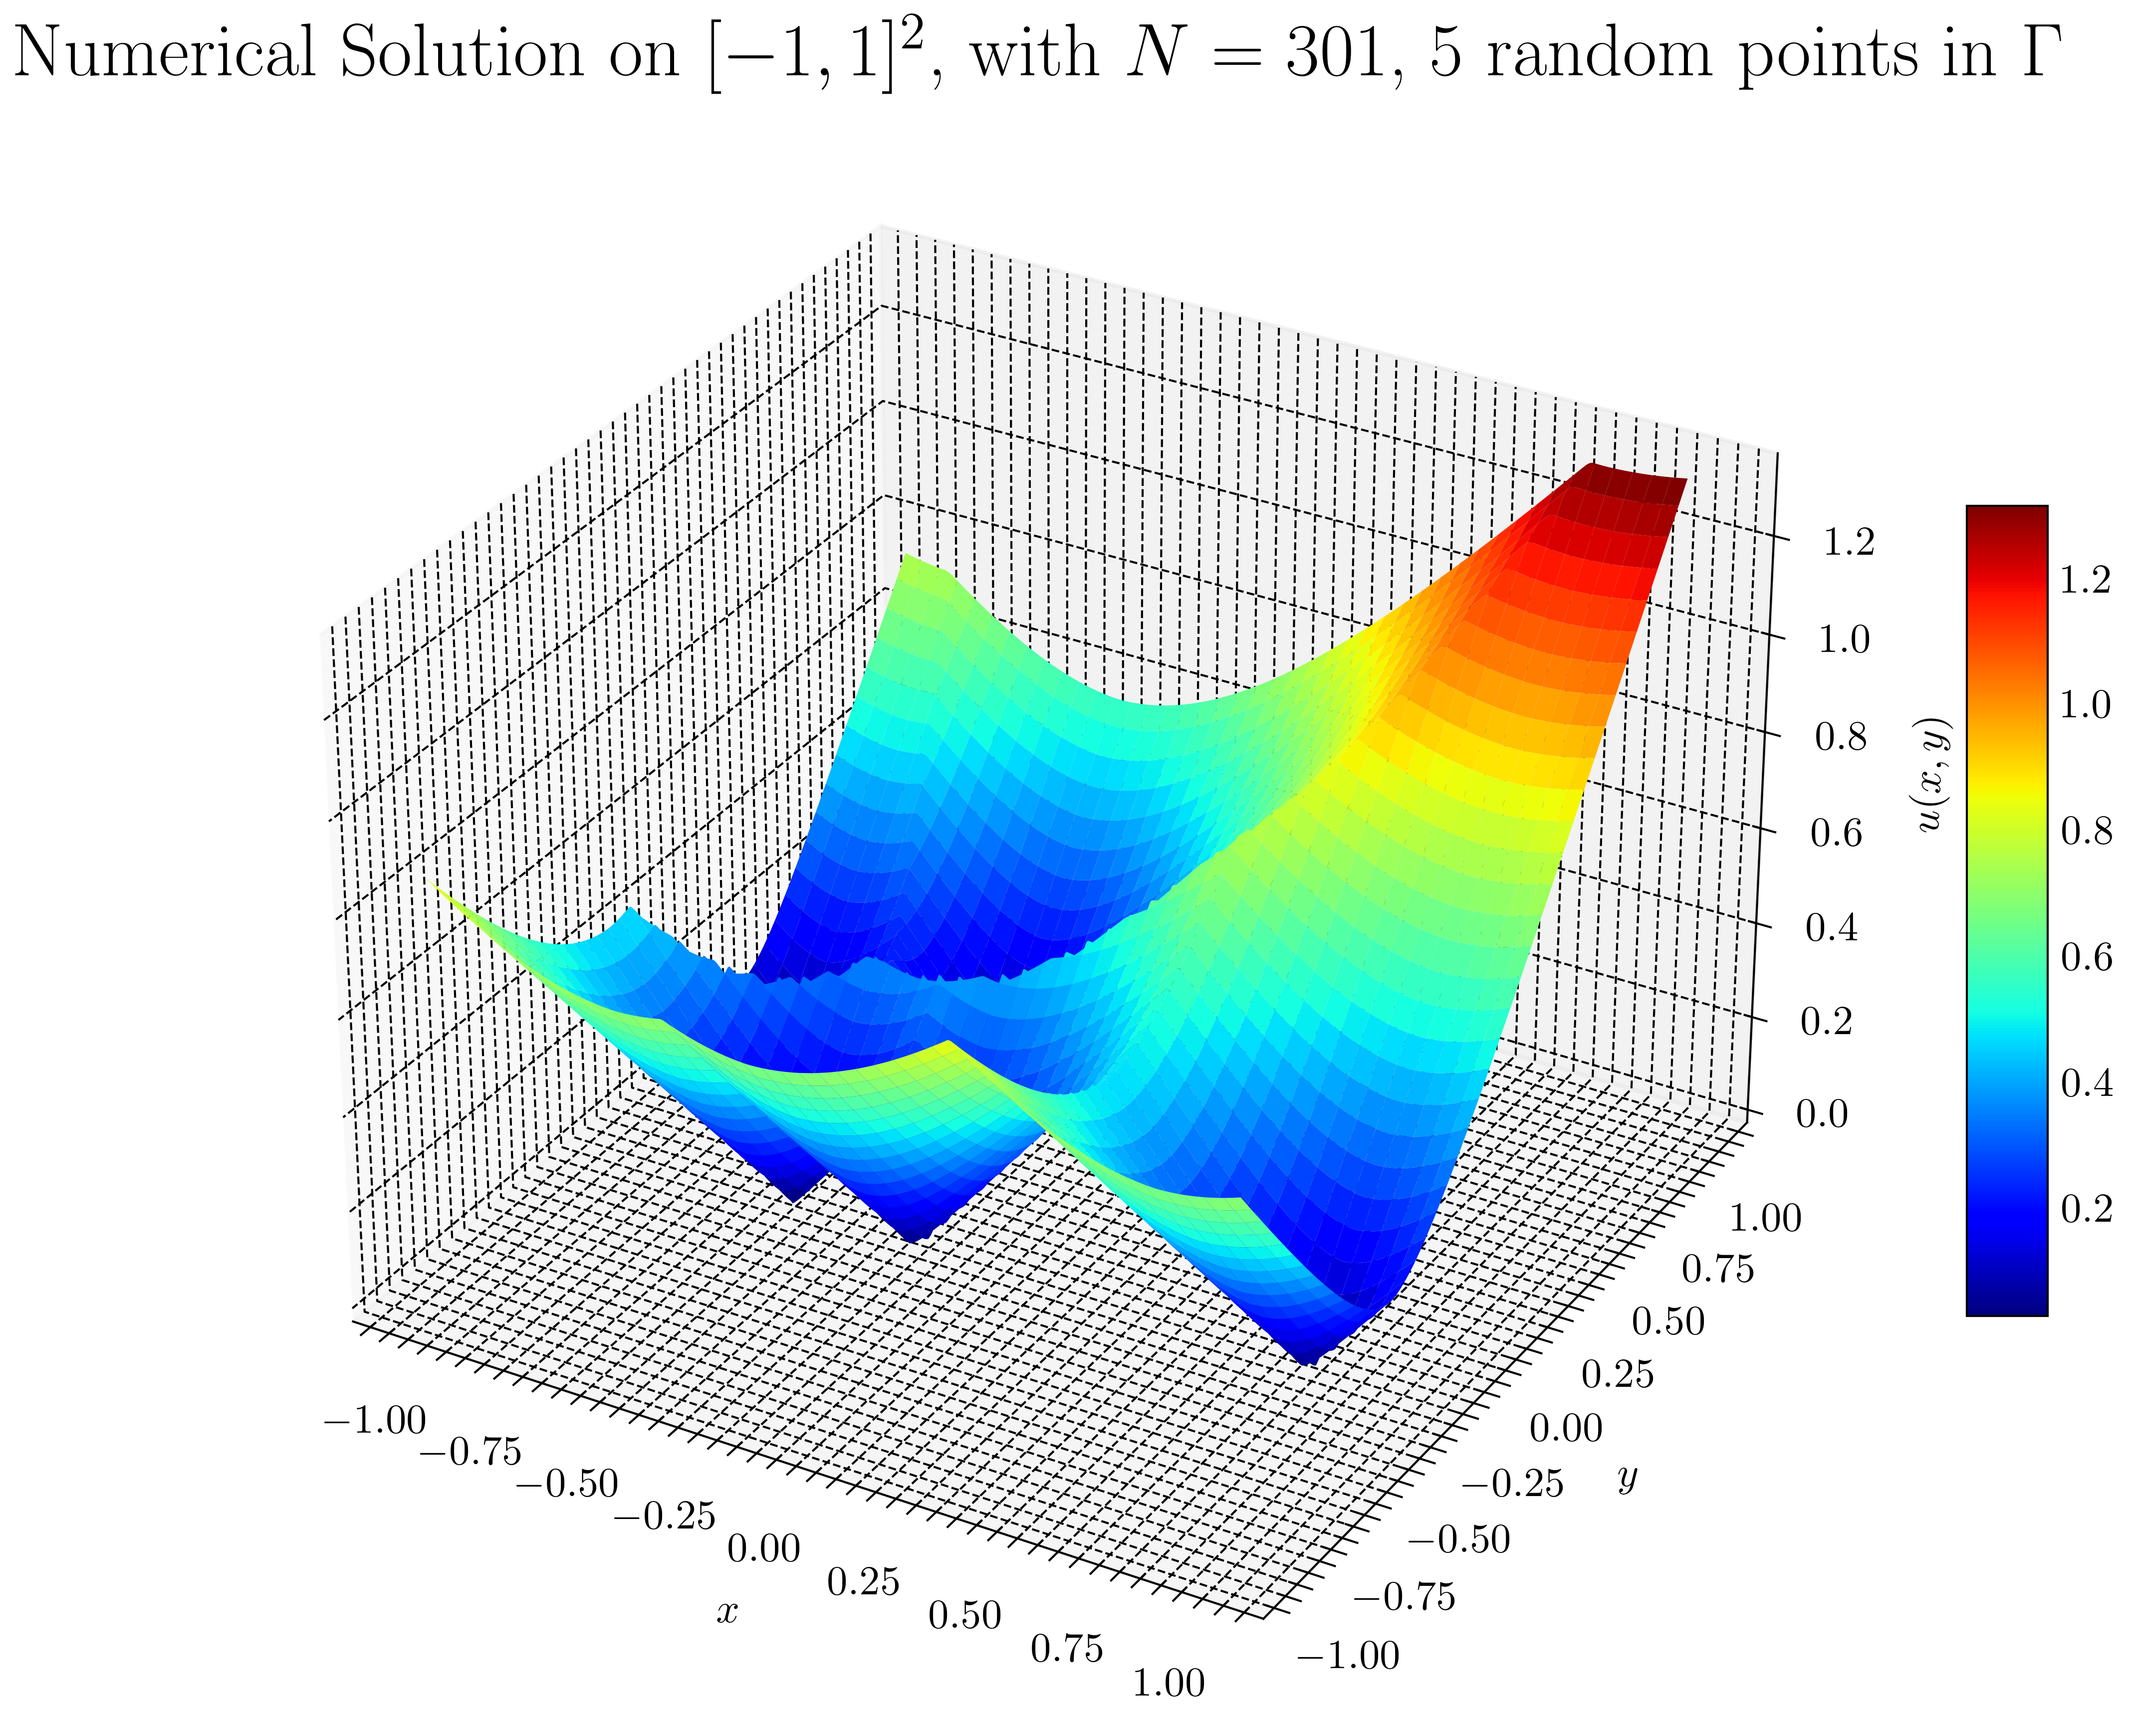
\includegraphics[width=\linewidth]{plots/solution_3d_surface_random5.png}
    \caption{3D surface of the solution ($|\Gamma$|=5)}
    \label{fig:surface5}
  \end{minipage}
\end{figure}


\newpage
\newpage
\section{Path planning}
In this section, we solve the following differential equation numerically in order to compute the shortest path.
\begin{equation}
    \frac{d\textbf{X}(t)}{dt}=-\nabla u(\textbf{X}(t))
\end{equation}
which ultimately leads us to the iteration 
\begin{equation}
    \textbf{X}_{k+1}=\textbf{X}_k-\Delta t \nabla \psi(\textbf{X}_k)
\end{equation}

THINGS TO ADD :
\begin{itemize}
    \item 2D distance : convergence plot, picture of the cone on the unit square, contour plots.
    \item 2D distance : random gamma : contour, heatmaps, 3d plot of the solution (argue on the discontinuities)
    \item 2D General F : equation that satisfies the PDE : compare with my solution (show number of iterations), 3d plots, contours
    \item 
    \item 
\end{itemize}
\end{document}

\end{document}
